\documentclass[utf8,english]{gradu3}
% If you are writing a Bachelor's Thesis, use the following instead:
%\documentclass[utf8,bachelor,english]{gradu3}

\usepackage{graphicx} % for including pictures

\usepackage{amsmath} % useful for math (optional)

\usepackage{booktabs} % good for beautiful tables

\usepackage{listings}

% NOTE: This must be the last \usepackage in the whole document!
\usepackage[bookmarksopen,bookmarksnumbered,linktocpage]{hyperref}

\graphicspath{ {img/} }
\addbibresource{bibliography.bib} % The file name of your bibliography database

\begin{document}

\title{Migrating a web application to serverless architecture}
\translatedtitle{Web-sovelluksen siirtäminen serverless-arkkitehtuuriin}
\studyline{Master's Thesis in Information Technology}
\avainsanat{%
  serverless,
  FaaS,
  arkkitehtuuri,
  pilvilaskenta,
  web-sovellukset}
\keywords{
  serverless,
  FaaS,
  architecture,
  cloud computing,
  web applications}
\tiivistelma{%
  Tämä kirjoitelma on esimerkki siitä, kuinka
  {gradu3}-tutkielmapohjaa käytetään.  Se sisältää myös
  käyttöohjeet ja tutkielman rakennetta koskevia ohjeita.

  Tutkielman tiivistelmä on tyypillisesti lyhyt esitys, jossa
  kerrotaan tutkielman taustoista, tavoitteesta, tutkimusmenetelmistä,
  saavutetuista tuloksista, tulosten tulkinnasta ja johtopäätöksistä.
  Tiivistelmän tulee olla niin lyhyt, että se, englanninkielinen
  abstrakti ja muut metatiedot mahtuvat kaikki samalle sivulle.

  Sen tulee kertoa täsmälleen samat asiat kuin englannikielinen
  abstrakti.
}
\abstract{%
  This document is a sample {gradu3} thesis document class
  document.  It also functions as a user manual and supplies
  guidelines for structuring a thesis document.

  The abstact is typically short and discusses the background, the
  aims, the research methods, the obtained results, the interpretation
  of the results and the conculsions of the thesis.  It should be so
  short that it, the Finnish translation, and all other meta
  information fit on the same page.

  The Finnish tiivistelmä of a thesis should usually say exactly the same
  things as the abstract.
}

\author{Aleksi Pekkala}
\contactinformation{\texttt{alvianpe@student.jyu.fi}}
% use a separate \author command for each author, if there is more than one
\supervisor{Oleksiy Khriyenko}
% use a separate \supervisor command for each supervisor, if there
% is more than one

\maketitle

% \begin{thetermlist}
% \item[FaaS] Function as a Service.
% % \item[\LaTeX] A system, built on top of \TeX\
% %   \parencite{knuth86:_texbook}, for typesetting structured
% %   documents \parencite[see][]{lamport94:_latex}.  Its current version
% %   is \LaTeXe.
% \end{thetermlist}

\mainmatter

\chapter{Introduction} \label{cha:introduction}

% TODO check preprints etc in bibliography

Cloud computing has in the past decade emerged as a veritable backbone of modern economy, driving innovation both in industry and academia as well as enabling scalable global enterprise applications. Just as the adoption of cloud computing continues to increase, the technologies in which the paradigm is based on have continued to progress. Recently the development of novel virtualization techniques has lead to the introduction of \textit{serverless computing}, an architectural pattern based on ephemeral cloud resources that scale up and down automatically and are billed for actual usage at a millisecond granularity. The main drivers behind serverless computing are both reduced operational costs through more efficient cloud resource utilization and improved developer productivity by shifting provisioning, load balancing and other infrastructure concerns to the platform. \parencite{buyya2017manifesto}

% TODO quote \textcite{mcgrath16cloudEventParadigms} "enormous potential as a disruptive cloud technology"

% TODO quote \textcite{jackson18languageImpact} Overall, the composition of functions in serverless appli- cations is a crucial design decision, which if done in an appropriately fine-grained manner, can lead to a more flexible but also more cost-effective solution in the long term, as functions can individually be implemented in the appropriate runtime to suit their purpose and expected throughput.

As an appealing economic proposition, serverless computing has attracted significant interest in the industry. This is illustrated for example by its appearance in the 2017 Gartner Hype Technologies Report \parencite{walker17gartnerHype}. By now most of the prominent cloud service providers have introduced their own serverless platforms, promising capabilities that make writing scalable web services easier and cheaper \parencite[e.g.][]{awslambda0218, google18cloudFunctions, ibm18cloudFunctions, microsoft18azureFunctions}. A number of high-profile use cases have also been presented in the literature \parencite{cncf18serverlessWG}. \textcite{baldini17currentTrends} however note a lack of corresponding degree of interest in academia despite a wide variety of technologically challenging and intellectually deep problems in the space.

One of the open problems identified in literature concerns the discovery of serverless design patterns: how do we compose the granular building blocks of serverless into larger systems? \parencite{baldini17currentTrends} \textcite{varghese18next} contend that one challenge hindering the widespread adoption of serverless will be the radical shift in the properties that a programmer will need to focus on, from latency, scalability and elasticity to those relating to the modularity of an application. Considering this and the paradigm's unique characteristics and limitations, it's unclear to what extent our current patterns apply and what kind of new patterns are best suited to optimize for the features of serverless computing. The object of this thesis is to fill the gap by re-evaluating existing design patterns in the serverless context and proposing new ones through an exploratory migration process.

\section{Research problem}

The research problem addressed by this thesis distills down to the following 4 questions:
\begin{enumerate}
	\item Why should a web application be migrated to serverless?
	\item What kind of patterns are there for building serverless web application backends?
	\item Do the existing patterns have gaps or missing parts, and if so, can we come up with improvements or alternative solutions?
	\item How does migrating a web application to serverless affect its quality?
\end{enumerate}

The first two questions are addressed in the theoretical part of the thesis. Question 1 concerns the motivation behind the thesis and introduces serverless migration as an important and relevant business problem. Question 2 is answered by surveying existing literature for serverless patterns as well as other, more general patterns thought suitable for the target class of applications.

The latter questions form the constructive part of the thesis. Question 3 concerns the application and evaluation of surveyed patterns. The surveyed design patterns are used to implement a subset of an existing conventional web application in the serverless architecture. In case the patterns prove unsuitable for any given problem, alternative solutions or extensions are proposed. The last question consists of comparing the migrated portions of the app to the original version and evaluating whether the posited benefits of serverless architecture are in fact realized.

\section{Outline}

The thesis is structured as follows: the second chapter serves as an introduction to the concept of serverless computing. The chapter describes the main benefits and drawbacks of the platform, as well as touching upon its internal mechanisms and briefly comparing the main service providers. Extra emphasis is placed on how the platform's limitations should be taken into account when designing web application backends.

The third chapter consists of a survey into existing serverless design patterns and recommendations. Applicability of other cloud computing, distributed computing and enterprise integration patterns is also evaluated.

The fourth chapter describes the process of migrating an existing web application to serverless architecture. The patterns discovered in the previous chapter are utilized to implemented various typical web application features on a serverless platform. In cases where existing patterns prove insufficient or unsuitable as per the target application's characteristics, modifications or new patterns are proposed.

The outcome of the migration process is evaluated in the fifth chapter. The potential benefits and drawbacks of the serverless platform outlined in chapter 2 are used to reflect on the final artifact. The chapter includes approximations on measurable attributes such as hosting costs and performance as well as discussion on the more subjective attributes like maintainability and testability. The overall ease of development -- or developer experience -- is also addressed since it is one of the commonly reported pain points of serverless computing \parencite{van2017spec}.

The final chapter of the thesis aims to draw conclusions on the migration process and the resulting artifacts. The chapter contains a summary of the research outcomes and ends with recommendations for further research topics.

\chapter{Serverless computing} \label{cha:serverless}

This chapter serves as an introduction to serverless computing. Defining serverless computing succinctly can be difficult because of the relative immaturity of the field. The NIST definitions of cloud computing have yet to catch up with the technology \parencite{nist11definitions}, and an effort to formalize and standardize serverless computing by the industry-headed Cloud Native Computing Foundation is still underway \parencite{cncf18serverlessWG} TODO whitepaper now released. As a result the boundaries between serverless and other cloud computing terms are still somewhat blurred, and the terms seem to carry slightly different meanings depending on the author or context. To complicate matters further, serverless computing has come to appear in two different but overlapping forms. A multilayered approach is therefore in order.

We approach the formidable task of defining serverless by first taking a brief look at the history and motivations behind utility computing. After that we'll introduce the basic tenets of serverless computing, distinguish between its two main approaches and see how it positions itself relative to other cloud service models. This is followed by a more technical look at the most recent serverless model, as well as its major providers, use cases, security issues and economic implications. The chapter closes with notes on the drawbacks and limitations of serverless, particularly from the point of view of web application backends. This thesis' definition of serverless leans heavily on the CNCF Serverless Working Group's whitepaper \parencite{cncf18serverlessWG}, the seminal introduction to the topic by \textcite{robert2016serverlessarchitectures} as well as a number of recent survey articles \parencite[e.g.][]{baldini17currentTrends,van2017spec,fox17}

As a sidenote, although earliest uses of the term 'serverless' can be traced back to peer-to-peer and client-only solutions \parencite{fox17}, we're dismissing these references since the name has evolved into a completely different meaning in the current cloud computing context. As per \textcite{robert2016serverlessarchitectures}, first usages of the term referring to elastic cloud computing seem to have appeared at around 2012.

% TODO: How does serverless relate to concepts such as FaaS, BaaS/MBaaS like Auth0 and Firebase, SOA, microservices, event-driven, virtualization, containers, cloud-native, ...? Cloud-ready/cloud-native as defined by \textcite{pozdniakova17cloudready}.

\section{Background} \label{sec:background}

Utility computing refers to a business model where computing resources, such as computation and storage, are commoditized and delivered as metered services in a similarly to physical public utilities such as water, electricity and telephony. Utilities are readily available to consumers at any time whenever required and billed per actual usage. In computing, this has come to mean on-demand access to highly scalable subscribtion-based IT resources. The availability of computing as an utility enables organizations to avoid investing heavily on building and maintaining complex IT infrastructure. \parencite{buyya09cloud}

This vision of utility computing can be traced all the way back to 1961, with the computing pioneer John McCarthy predicting that ``computation may someday be organized as a public utility'' \parencite{foster08cloudGrid}. Likewise in 1969 Leonard Kleinrock, one of the chieft scientists in the ARPANET project, is quoted as saying, ``as of now, computer networks are still in their infancy, but as they grow up and become sophisticated, we will probably see the spread of ‘computer utilities’ which, like present electric and telephone utilities, will service individual homes and offices across the country'' \parencite{kleinrock03internet}. The creation of the Internet first facilitated weaving computer resources together into large-scale distributed systems. Onset by this discovery, multiple computing paradigms have been proposed and adopted over the years to take on the role of a ubiquitous computing utility, including cluster, grid, peer-to-peer (P2P) and services computing \parencite{buyya09cloud}. The latest paradigm, cloud computing, has in the past decade revolutionized the computer science horizon and got us closer to computing as an utility than ever \parencite{buyya2017manifesto}.

\textcite{sareen13cloudTypes} succinctly defines the cloud as ``a pool of virtualized computer resources''. \textcite{foster08cloudGrid} present a more thorough definition of cloud computing as ``a large-scale distributed computing paradigm that is driven by economies of scale, in which a pool of abstracted, virtualized, dynamically-scalable, managed computing power, storage, platforms, and services are delivered on demand to external customers over the Internet''. Cloud computing builds on the earlier paradigm of grid computing, and relies on grid computing as its backbone and infrastructure. Compared to infrastructure-based grid computing, cloud computing focuses on more abstract resources and services. \textcite{buyya2017manifesto} also note that cloud computing differs from grid computing in that it
promises virtually unlimited computational resources on demand.

% expound on IaaS/PaaS/SaaS here?

The first cloud providers were born out of huge corporations offering their surplus computing resources as a service in order to offset expenses and improve utilization rates. Having set up global infrastructure to handle peak demand, a large part of the resources were left under-utilized at times of average demand. The providers are able to offer these surplus resources at attractive prices due to the large scale of their operations, benefiting from economies of scale. To address consumers' concerns about outages and other risks, cloud providers guarantee a certain level of service delivery through Service Level Agreements (SLA) that are negotiated between providers and consumers. \parencite{youseff08cloudOntology}

The key technology that enables cloud providers to transparently handle consumers' requests without impairing their own processing needs is \textit{virtualization}. Virtualization is one of the main components behind cloud computing and one of the factors setting it apart from grid computing. \textcite{sareen13cloudTypes} defines virtualization as using computer resources to imitate other computer resources or whole computers. This enables the abstraction of the underlying physical resources as a set of multiple logical virtual machines (VM). Virtualization has three characteristics that make it ideal for cloud computing: 1) \textit{partitioning} supports running many applications and operating systems in a single physical system; 2) \textit{isolation} ensures boundaries between the host physical system and virtual containers; 3) \textit{encapsulation} enables packaging virtual machines as complete entities to prevent applications from interfering with each other.
% foster08 has more on virtualization

Virtual machines manage to provide strong security guarantees by isolation, i.e., by allocating each VM its own set of resources with minimal sharing between the host system. Minimal sharing however translates into high memory and storage requirements as each virtual machine requires a full OS image in addition to the actual application files. A virtual machine also has to go through the standard OS boot process on startup, resulting in launching times measured in minutes. Rapid innovation in the cloud market and virtualization technologies has recently lead to an alternative, more lightweight \textit{container}-based solution. Container applications share a kernel with the host, resulting in significantly smaller deployments and fast launching times ranging from less than a second to a few seconds. Due to resource sharing a single host is capable of hosting hundreds of containers simultaneously. Differences in resource sharing between VM- and container-based deployment is illustrated in figure \ref{fig:vmVsContainer}. As a downside containers lack the VM's strong isolation guarantee and the ability to run a different OS per deployment. On the other hand, containers provide isolation via namespaces, so processes inside containers are still isolated from each other as well as the host. \textit{Containerization} has emerged as a common practice of packaging applications and related dependencies into standardized container images to ease development efficiency and interoperability. \parencite{pahl15containerization}
% mention CaaS, kubernetes etc
% he container technology due to its small footprint and fast deployment is crucial in serverless

\begin{figure}[h]
  \centering
  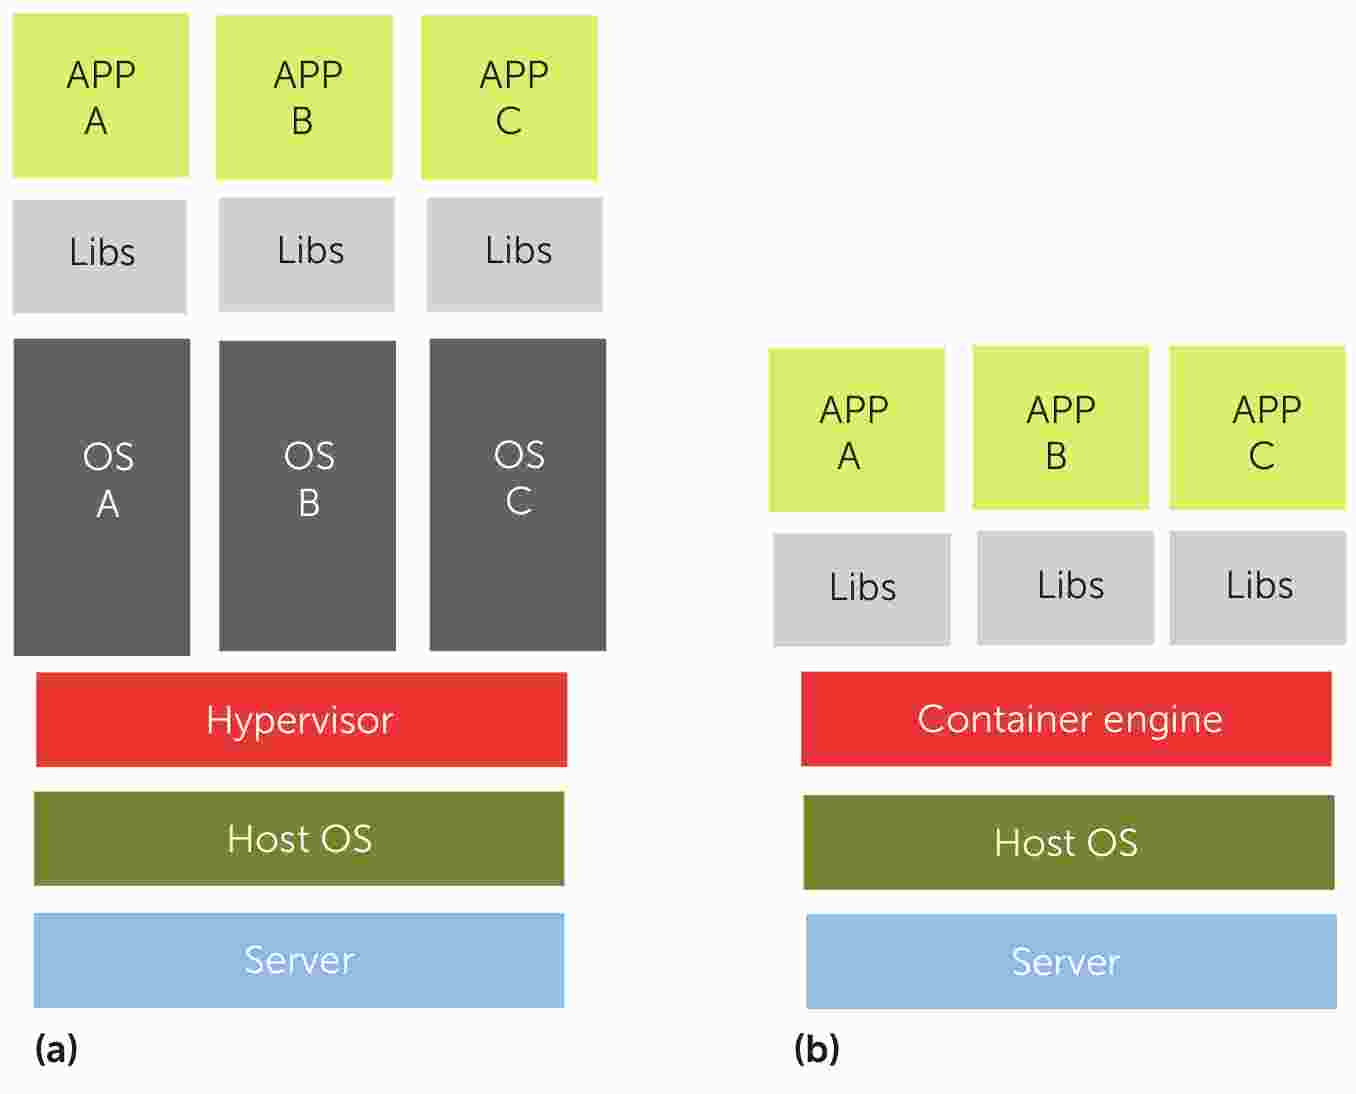
\includegraphics[width=0.8\textwidth]{bernstein14-vm-vs-container.jpg}
  \caption{Comparison of a) virtual machine- and b) container-based deployments \parencite{bernstein14containers}}
  \label{fig:vmVsContainer}
\end{figure}

Cloud computing is by now a well-established paradigm that enables organizations to flexibly deploy a wide variety of software systems over a pool of externally managed computing resources. Both major IT companies and startups see migrating on-premise legacy systems to the cloud as an opportunistic business strategy for gaining competetive advantage. Cost savings, scalability, reliability and efficient utilization of resources as well as flexibility are identified as key drivers for migrating applications to the cloud \parencite{jamshidi13cloudmigrationreview}. However, although the state-of-the-art in cloud computing has advanced significantly over the past decade, several challenges remain.
% Thus, Cloud computing has enabled new businesses to establish in a shorter amount of time, has facilitated the expansion of enterprises across the globe, has accelerated the pace of scientific progress, and has led to the creation of various models of computation for pervasive and ubiquitous applications, among other benefits.

One of the open issues in cloud computing concerns pricing models. In the current cloud service models pricing typically follows the ``per instance per hour'' model; that is, the consumer is charged for the duration that an application is hosted on a VM or a container \parencite{varghese18next}. The flaw in this model is that idle time is not taken into account. Whether the application was used or not doesn't have an effect: the consumer ends up paying for the whole hour even if the application was actually performing computation for just a couple of seconds. This makes sense from the provider's point of view, since for the duration billed, the instance is provisioned and dedicated solely to hosting the consumer's application. However, paying for idle time is of course undesirable for the consumer, and the problem is made worse in case of applications with fluctuating and unpredictable workloads.

Continuously hosting non-executing applications is problematic on the provider side as well as it leads to under-utilization. Just as consumers end up paying for essentially nothing, providers end up provisioning and tying up resources to do essentially nothing. Fundamentally the problem of under-utilization boils down to elasticity and resource management. The current cloud computing models are incapable of automatically scaling up and down to meet current demand while at the same time maintaining their stringent Quality-of-Service (QoS) expectations \parencite{buyya2017manifesto}. Lacking automatic scaling mechanisms, cloud consumers are left to make capacity decisions on their own accord, and as \textcite{robert2016serverlessarchitectures} notes, consumers typically err on the side of caution and over-provision. This in in turn leads to inefficiencies and under-utilization as described above.

% On one hand, a pay-per-use model only brings cost savings with respect to a dedicated (statically sized) system solution if (1) an application has varying load over time and (2) the application provider is able to allocate the “right” amount of resources to it, avoiding both over-provisioning (paying for unneeded resources) and under-provisioning resulting in QoS degradation. On the other hand, years of cloud development experience have taught practitioners that commodity server hardware and network switches break often. Failure domains help isolate problems, but one should “plan for failure”, striving to produce resilient applications on unreliable infrastructure, without compromising their elastic scalability.

The problem of low utilization rates in data centers is particularly relevant in the current energy-constrained environment. ICT in general consumes close to 10\% of all electricity world-wide, with the CO$_2$ impact comparable to air travel \parencite{buyya2017manifesto}. It's estimated that in 2010 data centers accounted for 1-2\% of global energy usage, with data center carbon emissions growing faster than the annual global footprint as well as the footprint of other ICT subcategories. While data centers are improving in energy efficiency, so is the demand for computing services with both the magnitude of data produced and complexity of software increasing. Operational factors such as excessive redundancy also affect data center energy efficiency heavily. A survey of Google data centers -- considered to represent the higher end of utilization -- revealed utilization of 60\% or less 95\% of the time and 30\% or less half of the time. Another analysis found that data centers spend on average only 6\% to 12\% of the electricity powering servers that do computation, with the rest used to keep servers idling for redundancy. \parencite{horner16powerusage}

% In addition to increasing demand for computation and storage resources we've seen an increase in software complexity. To address the problem of software complexity we've seen an evolution of architecture patterns from monolith to SOA to microservices... The major disadvantage of the microservice model as illustrated in the previous example is that we still need to provision a cluster of compute resources to run the services, then manage and scale these compute resources \parencite{gannon17cloudNative}
% {balalaie16migratingcloud} talk about the reasons behind migrating systems to cloud-native architectures; cloud-native architectures that consider availability and scaling have to be utilized to fully benefit from cloud migration

Cloud computing, having ``revolutionized the computer science horizon and enabled the emergence of computing as the fifth utility'' \parencite{buyya2017manifesto}, will face considerable new requirements in the coming decade. It's predicted that by 2020 over 20 billion sensor-rich devices like phones and wearables will be connected to the Internet generating trillions of gigabytes of data. \textcite{varghese18next} argue that increasing volumes of data pose significant networking and computing challenges that cannot be met by existing cloud infrastructure, and that adding more centralized cloud data centers will not be enough to address the problem. The authors instead call for new computing models beyond conventional cloud computing, one of which is serverless computing.

\section{Defining serverless} \label{sec:definingServerless}

%Serverless platforms promise new capabilities that make writing scalable microservices easier and cost effective, positioning themselves as the next step in the evolution of cloud computing architectures. \parencite{baldini17currentTrends}
% serverless takes these benefits to the extreme... how does serverless lean on the prev mentioned technology, compare to other platforms. link to prev section!
% FaaS poses new challenges particularly for resource management in Clouds that will need to be addressed. This is because arbitrary code (the function) will need to execute in the Cloud without any explicit specifi- cation of resources required for the operation. To make this possible, FaaS providers pose many restrictions about what functions can do and for how long they can operate [16]. For example, they enforce limits on the amount of time a function can execute, how functions can be written, and how the code is deployed [16]. This is restrictive in the types of applications that can make use of current FaaS models. The adoption of the FaaS model will however increase if a wider range of applications can make use of restriction relaxed FaaS models, which will evolve what is now a ”niche” service model to an effective method for developing Cloud applications.

% Serverless computing is a style of cloud computing where you write code and define the events that should cause the code to execute and leave it to the cloud to take care of the rest. There is another type of cloud service that is related to serverless concept. These are called “fully managed” services because the service manages all of the infrastructure resourcing, management, and scaling, along with the workflow needed to carry out your computation. There is no need for the user to allocate resources. For example, Azure CosmosDB allows a user to add their own functions and proce- dures to their databases. These functions are exe- cuted by triggers or by user queries. We can compose fully managed services to build new applications that have all the properties we require of cloud-native. \parencite{gannon17cloudNative}

TODO: link to previous section, present serverless as in many ways the next reductive step in IaaS to PaaS abstraction. Explain figure \ref{fig:serverlessLineage} \parencite{van18fromPAAStoPresent}.

\begin{figure}[h]
  \centering
  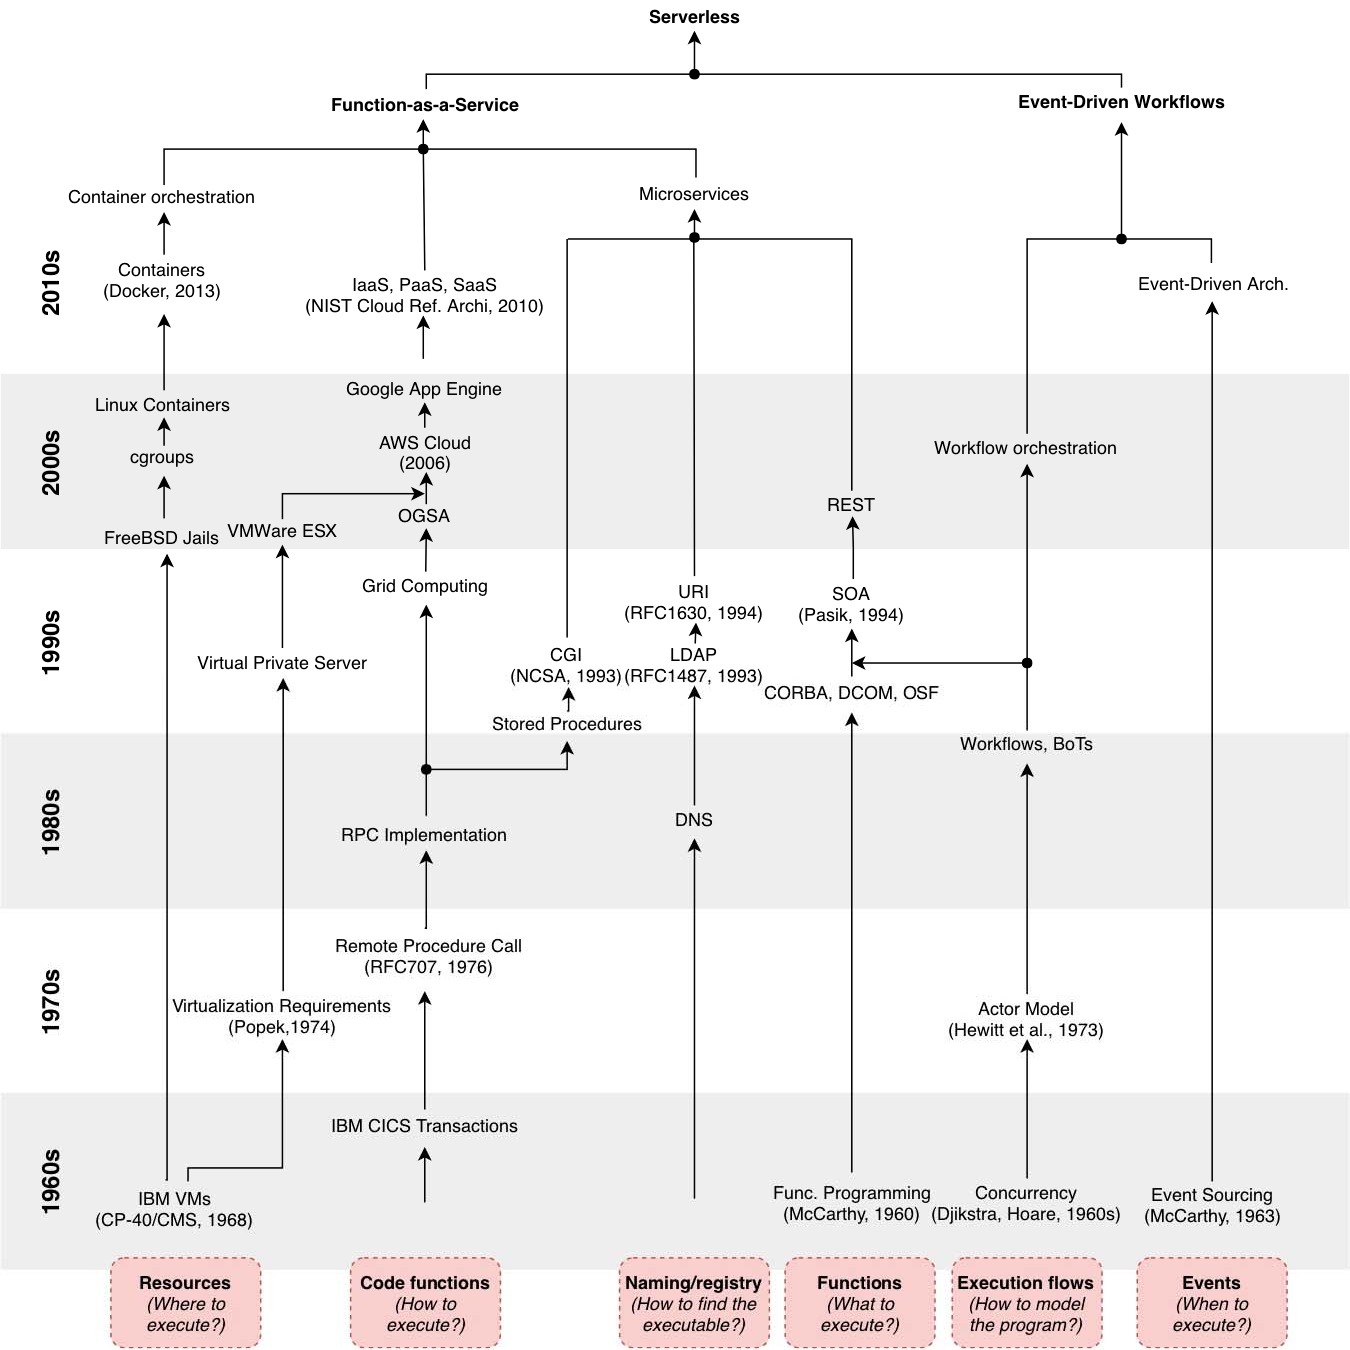
\includegraphics[width=0.9\textwidth]{eyk18-serverless-lineage.png}
  \caption{A history of computer science concepts leading to serverless computing \parencite{van18fromPAAStoPresent}}
  \label{fig:serverlessLineage}
\end{figure}

Fundamentally serverless computing is about building and running back-end code that does not require server management or server applications. The term itself can seem a bit disingenuous, since despite the name serverless computing obviously still involves servers. The name -- coined by industry -- instead carries the meaning that the resources used by the application are managed by the cloud service provider. As tasks such as provisioning, maintenance and capacity planning are outsourced to the serverless platform, developers are left to focus on application logic. For the cloud customer this provides an abstraction where computation is disconnected from the infrastructure it is going to run on. \parencite{robert2016serverlessarchitectures,cncf18serverlessWG}

\textcite{van2017spec} further define serverless computing by three key characteristics: \begin{enumerate}
  \item Granular billing: the user of a serverless model is charged only when the application is actually executing
  \item (Almost) no operational logic: operational logic, such as resource management and autoscaling, is delegated to the infrastructure, making those concerns of the infrastructure operator
  \item Event-driven: interactions with serverless applications are designed to be short-lived, allowing the infrastructure to deploy serverless applications to respond to events, so only when needed
\end{enumerate}

TODO: link to SOA and microservices: ``We see the emerging model based on running individual cloud functions as a consequence of the slow but sustained evolution of computing. For many decades we have witnessed a transition from relatively large, monolithic applications, to smaller or more structured applications with smaller execution units (e.g, workflows with many small tasks). This transition is captured qualitatively by various software architectures, for example, the Service-Oriented Architecture, and quantitatively by various workload-characterization and modeling studies, for example of scientific workloads running on supercomputers and grids between 1990 and 2010.'' \parencite{van2017spec} Also \textcite{forrester16microservices} with ``Microservices lead to a serverless'' and \textcite{villamizar2016infrastructure} on SOA.

TODO: link to the event-driven paradigm: ``Serverless computing is a partial realization of an event-driven ideal, in which applications are defined by actions and the events that trigger them. This language is reminiscent of active database systems, and the event-driven literature has theorized for some time about general computing systems in which actions are processed reactively to event streams. Serverless function platforms fully embrace these ideas, defining actions through simple function abstractions and building out event processing logic across their clouds.'' \parencite{schmidt08event}

Serverless computing has in effect come to encompass two distinct cloud computing models: Backend-as-a-Service (BaaS) as well as Function-as-a-Service (FaaS). The two serverless models, while different in operation as explained below, are nonetheless grouped under the same serverless umbrella since they deliver the same main benefits: zero server maintenance overhead and the elimination of idle costs. \parencite{cncf18serverlessWG}

Backend-as-a-Service refers to an architecture where an application's server-side logic is replaced with external, fully managed cloud services that carry out various tasks like authentication or database access \parencite{buyya2017manifesto}. The model is typically utilized in the mobile space to avoid having to manually set up and maintain server resources for the more narrow back-end requirements of a mobile application. In the mobile context this form of serverless computing is also referred to as Mobile-Backend-as-a-Service (MBaaS) \parencite{sareen13cloudTypes}. The application's core business logic is implemented client-side and integrated tightly with third party remote application services. Since these API-based BaaS services are managed transparently by the cloud service provider, the model appears to the developer to be serverless.

Function-as-a-Service is defined in a nutshell as ``a style of cloud computing where you write code and define the events that should cause the code to execute and leave it to the cloud to take care of the rest'' \parencite{gannon17cloudNative}. In the FaaS architecture an application's business logic is still located server-side. The crucial difference is that instead of self-managed server resources, developers upload small units of code to a FaaS platform that executes the code in short-lived, stateless compute containers in response to events \parencite{robert2016serverlessarchitectures}. The model appears serverless in the sense that the developer has no control over the resources on which the back-end code runs. \textcite{albuquerque17faaspaas} note that the BaaS model of locating business logic on the client side carries with it some complications, namely difficulties in updating and deploying new features as well as reverse engineering risks. FaaS circumvents these problems by retaining business logic server-side.

Out of the two serverless models FaaS is a more recent development: the first commercial FaaS platform, AWS Lambda, was introduced in November 2014 \parencite{awslambda0218}.
FaaS is also the model with significant differences to traditional web application architecture \parencite{robert2016serverlessarchitectures}. These differences and their implications are further illustrated in section \ref{sec:processingModel}. As the more novel architecture, FaaS is especially relevant to the research questions in hand and is thus paid more attention in the remainder of this thesis.

Another perspective on the difference between the two serverless models is to view BaaS as a more tailored, vendor-specific approach to FaaS \parencite{van2017spec}. Whereas BaaS-type services function as built-in components for many common use cases such as user management and data storage, a FaaS platform allows developers to implement more customized functionality. BaaS plays an important role in serverless architectures as it will often be the supporting infrastructure (e.g. in form of data storage) to the stateless FaaS functions \parencite{cncf18serverlessWG}. Conversely, in case of otherwise BaaS-based applications there's likely still a need for custom server-side functionality; FaaS functions may be a good solution for this \parencite{robert2016serverlessarchitectures}. Serverless applications can utilize both models simultaneously, with BaaS platforms generating events that trigger FaaS functions, and FaaS functions acting as a 'glue component' between various third party BaaS components. \textcite{robert2016serverlessarchitectures} also notes convergence in the space, giving the example of the user managemement provider Auth0 starting initially with a BaaS-style offering but later entering the FaaS space with a 'Auth0 Webtask' service.

It's worth noting that not all authors follow this taxonomy of FaaS and BaaS as the two subcategories of a more abstract serverless model. \textcite{baldini17currentTrends} explicitly raise the question on whether serverless is limited to FaaS or broader in scope, identifying the boundaries of serverless as an open question. Some sources \parencite[][among others]{hendrickson16openlambda,mcgrath17implement,varghese18next} seem to strictly equate serverless with FaaS, using the terms synonymously. Considering however that the term 'serverless' predates the first FaaS platforms by a couple of years \parencite{robert2016serverlessarchitectures}, it seems sensible to at least make a distinction between serverless and FaaS. In this thesis we'll stick to the \textcite{cncf18serverlessWG} definition as outlined above.

\section{Comparison to other cloud computing models} \label{sec:comparisonCloud}

% As serverless is gaining popularity the boundaries between different types of ”as-a-Service” may be disappearing (see Figure 9). One could imagine that developers not only write code but also declare how they want the code to run - as FaaS orMBaaS or PaaS - and can change as needs change. In the future the main distinction may be between caring about server (server-aware) and not caring about server details (server-less). PaaS is in the middle; it makes it very easy to deploy code but developers still need to know about servers and be aware of scaling strategies, such as how many instances to run. \parencite{baldini17currentTrends}

Another approach to defining serverless is to compare it with other cloud service models. The commonly used NIST definition divides cloud offerings into three categories: Infrastructure-as-a-Service (IaaS), Platform-as-a-Service (PaaS) and Software-as-a-Service (SaaS), in order of increasing degree of abstraction of cloud infrastructure \parencite{nist11definitions}. On this spectrum serverless computing positions itself in the space between PaaS and SaaS, as illustrated in figure \ref{fig:degreeOfAutomation} \parencite{baldini17currentTrends}. Figure \ref{fig:cloudSpectrum} illustrates how the two serverless models relate, with the cloud provider taking over a larger share of operational logic in BaaS. \textcite{van2017spec} note that there's some overlap and give examples of non-serverless products in both the PaaS and SaaS worlds that nonetheless exhibit the main characteristics of serverless defined in section \ref{sec:definingServerless}.
% TODO flesh out this paragraph (explain IaaS etc as per buyya17?)

\begin{figure}[h]
  \centering
  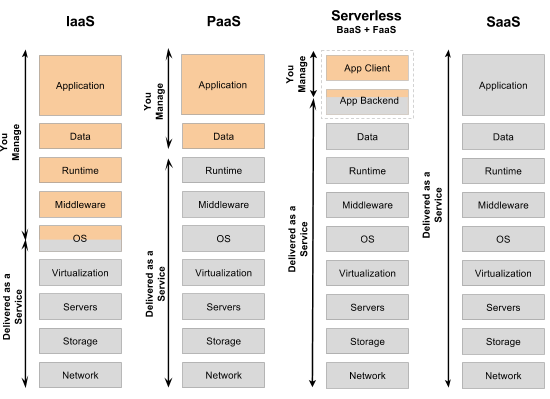
\includegraphics[width=0.9\textwidth]{specify-io-cloud-comparison.png}
  \caption{Degree of automation when using serverless \parencite{wolf16serverless}}
  \label{fig:degreeOfAutomation}
\end{figure}

\begin{figure}[h]
  \centering
  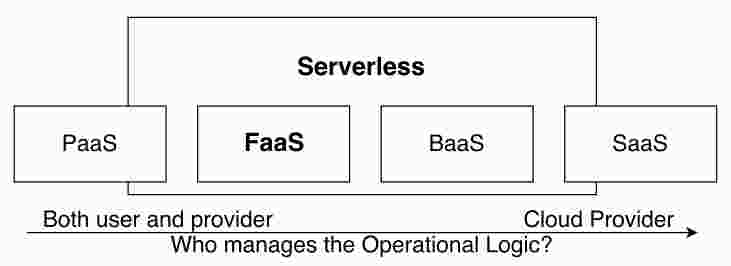
\includegraphics[width=0.8\textwidth]{eyk17-cloud-comparison.jpg}
  \caption{Serverless and FaaS vs. PaaS and SaaS \parencite{van2017spec}}
  \label{fig:cloudSpectrum}
\end{figure}

Since the gap between PaaS and FaaS can be quite subtle it warrants further consideration. Indeed some sources \parencite[e.g.][]{adzic2017serverless} refer to FaaS as a new generation of PaaS offerings. Both models provide a high-level and elastic computing platform on which to implement custom business logic. There are however a number of substantial differences between the two models, which ultimately boil down to PaaS being an instance-based model with multiple server processes running on always-on server instances, as opposed to the on-demand resource allocation of FaaS. Put another way, ``most PaaS applications are not geared towards bringing entire applications up and down for every request, whereas FaaS platforms do exactly this'' \parencite{robert2016serverlessarchitectures}.

\textcite{albuquerque17faaspaas} derive a number of specific differences between PaaS and FaaS in their comparative analysis. First of all the units of deployment vary: PaaS applications are deployed as services, compared to the more granular function-based deployment of FaaS. Second, PaaS instances are always running whereas serverless workloads are executed on-demand. Third, PaaS platforms, although supporting auto-scaling to some extent, require the developer to explicitly manage the scaling workflow and number of minimum instances. FaaS on the other hand scales transparently and on-demand without any need for resource pre-allocation. Perhaps the most important distinction lies in billing: PaaS is billed by instantiated resources whether they're used or not, whereas FaaS is billed per-event only for the execution duration. The analysis concludes that PaaS is well suited for predictable or constant workloads with long or variable per-request execution times; FaaS in turn provides better cost benefit for unpredictable or seasonal workloads with short per-request execution times. It's also to be noted that PaaS doesn't suffer from limits on execution duration and many other restrictions of FaaS as described in section \ref{sec:limitations}.

Another recent cloud-native technology is Container-as-a-Service (CaaS)... \parencite{robert2016serverlessarchitectures, buyya2017manifesto}
% compare to CaaS \parencite{cncf18serverlessWG}. Buyya17 describes containers. \textcite{robert2016serverlessarchitectures} also has a few words on the topic: scaling and Reduced packaging and deployment complexity

\section{Serverless processing model} \label{sec:processingModel}

The \textcite{cncf18serverlessWG} whitepaper divides a generalized serverless solution into four constituents, as illustrated in figure \ref{fig:processingModel}:

\begin{itemize}
  \item Event sources - trigger or stream events into one or more function instances
  \item Function instances - a single function/microservice, that can be scaled with demand
  \item FaaS Controller- deploy, control and monitor function instances and their sources
  \item Platform services - general cluster or cloud services (BaaS) used by the FaaS solution
\end{itemize}

\begin{figure}[h]
  \centering
  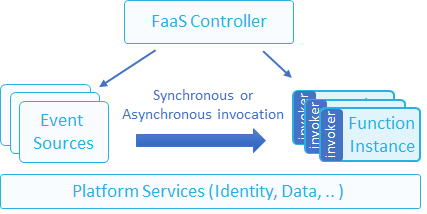
\includegraphics[width=0.8\textwidth]{cncf18-serverless-processing-model.png}
  \caption{Serverless processing model \parencite{cncf18serverlessWG}}
  \label{fig:processingModel}
\end{figure}

Interrelation of the various parts is further demonstrated with an example of a typical serverless development workflow. First, the developer selects a runtime environment (e.g. Python 3.6), writes a piece of code and uploads it on a FaaS platform where the code is published as a serverless function. The developer then maps one or more event sources to trigger the function, with event sources ranging from HTTP calls to database changes and messaging services. Now when any of the specified events occurs, the FaaS ontroller spins up a container, loads up the function along with its dependencies and executes the code. The function code typically contains API calls to external BaaS resources to handle data storage and other integrations. When there are multiple events to respond to simultaneously, more copies of the same function are run in parallel. Serverless functions thus scale precisely with the size of the workload, down to the individual request. After execution the container is torn down. Later the developer is billed according to the measured execution time, typically in 100 millisecond increments. \parencite{awslambda0218}

At the heart of serverless architecture is the concept of a \textit{function} (also \textit{lambda function} or \textit{cloud function}). A function represents a piece of business logic executed in response to specified events. Functions are the fundamental building block from which to compose serverless applications. A function is defined as a small, stateless, short-lived, on-demand service with a single functional responsibility \parencite{van2017spec}. As discussed in section \ref{sec:background}, the technology underlying cloud computing has evolved from individual servers to virtual machines and containers. \textcite{hendrickson16openlambda} see the serverless function model as the logical conclusion of this evolution towards more sharing between applications (figure \ref{fig:evolutionOfSharing}).

\begin{figure}[h]
  \centering
  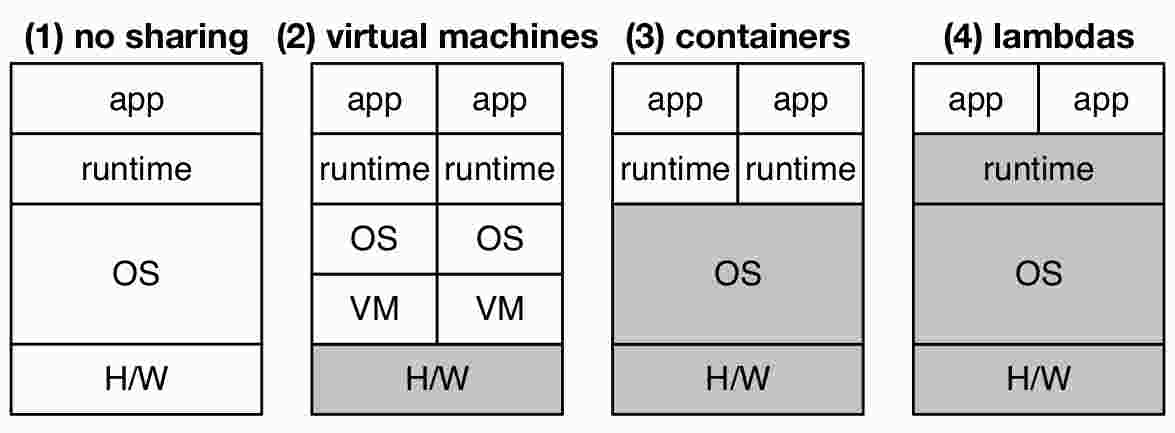
\includegraphics[width=0.8\textwidth]{hendrickson16-evolution-of-sharing.jpg}
  \caption{Evolution of sharing -- gray layers are shared \parencite{hendrickson16openlambda}}
  \label{fig:evolutionOfSharing}
\end{figure}

Being stateless and short-lived, serverless functions have fundamentally limited expressiveness compared to a conventional PaaS-hosted application. This is a direct result of being built to maximise scalability. A FaaS platform will need to execute the arbitrary code in a function in response to any number of events, without explicitly specifying resources required for the operation \parencite{buyya2017manifesto}. To make this possible, FaaS platforms pose restrictions on what functions can do and how long they can operate. Statelessness here means that a function loses all local state after termination; none of the local state created during invocation will necessarily be available during subsequent invocations of the same function. This is where BaaS services come in, with external stateful services such as key-value stores, databases and file or blob storages providing a persistence layer. In addition to statelessness, FaaS platforms limit a funtion's execution duration and resource usage: AWS Lambda for example has a maximum execution duration of 15 minutes and a maximum memory allocation of 3008 MB \parencite{awslambda0218}.

FaaS event sources can be divided into two categories, synchronous and asynchronous. The first category follows a typical request-response flow: a client issues a request and blocks while waiting for a response. Synchronous event sources include HTTP and RPC calls which can be used to implement a REST API, a command line client or any other service requiring immediate feedback. Asynchronous event sources on the other hand result in non-blocking function execution, and they're typically used to implement background workers, scheduled event handlers and queue workers. Asynchronous event sources include message queues, publish-subscribe systems, database or file storage change feeds and CRON jobs among others. The details and metadata of the triggering event are passed to the function as an input parameter, with exact implementation varying per event type and provider. In case of a HTTP call, for example, the event object might include the request path, headers, body and query parameters. A function instance is also commonly supplied a context object, which in turn contains runtime information and other general properties that span multiple function invocations. Function name, version, memory limit and remaining execution time are examples of typical context variables. FaaS platforms also usually allow users to set environment variables which function instances can access through the context object -- useful for handling security keys and tokens. As for output, functions can either directly return a value (in case of synchronous invocation) or either trigger the next execution phase in a workflow or simply log the result (in case of asynchronous invocation). An example function handler is presented in listing \ref{lst:handlerExample}. In addition to publishing and executing serverless functions, FaaS platforms also typically provide auxiliary capabilities such as monitoring, statistics, versioning and logging. \parencite{cncf18serverlessWG}

\renewcommand\thelstlisting{\arabic{lstlisting}}
\setcounter{lstlisting}{0}
\begin{lstlisting}[language=Python,caption=Example FaaS handler,captionpos=b,label=lst:handlerExample,showstringspaces=false,belowskip=2em,frame=tb,aboveskip=2em]
  def main(event, context):
      return {"payload": "Hello, " + event.name}
\end{lstlisting}

As mentioned in section \ref{sec:definingServerless}, serverless is \textit{almost} but not completely devoid of operational management. In case of serverless functions, this qualification means that parameters such as memory reservation size, maximum parallelism and execution time are still left for the user to configure. Whereas the latter parameters are mainly used as safeguards to control costs, memory reservation size has important implications regarding execution efficiency \parencite{lloydserverless}. There are however tools available to determine the optimal memory reservation size per given workload. Also some platforms automatically reserve the required amount of memory without pre-allocation \parencite{microsoft18azureFunctions}.

% \textcite{fox17} present a useful short definition of a FaaS platform like Lambda as a cloud-native platform for short-running, stateless computation and event-driven applications which scales up and down instantly and automatically and charges for actual usage at a millisecond granularity.

Even with the restrictions on a serverless function's capabilities, implementing a FaaS platform is a difficult problem. From the customer's point of view the platform has to be as fast as possible in both spin-up and execution time, as well as scale indefinitely and transparently. The provider on the other hand seeks maximum resource utilization at minimal costs while avoiding violating the consumer's QoS expectations. Given that these goals are in conflict with each other, the task of resource allocation and scheduling bears crucial importance \parencite{reza17controller}. A FaaS platform must also safely and efficiently isolate functions from each other, and make low-latency decisions at the load balancer-level while considering session, code, and data locality \parencite{hendrickson16openlambda}.

\section{Use cases} \label{sec:useCases}

Serverless computing has been utilized to support a wide range of applications. \textcite{baldini17currentTrends} note that from a cost perspective, the model is particularly fitting for bursty, CPU-intensive and granular workloads, as well as applications with sudden surges of popularity such as ticket sales. Serverless is less suitable for I/O-bound applications where a large period of time is spent waiting for user input or networking, since the paid-for compute resources go unused. In the industry, serverless is gaining traction primarily in three areas: Internet-of-Things (IoT) applications with sporadic processing needs, web applications with light-weight backend tasks, and as glue code between other cloud computing services \parencite{spillner18faaster}.

A number of real-world and experimental use cases exists in literature. \textcite{adzic2017serverless} present two industrial case studies implementing mind-mapping and social networking web applications in serverless architectures, resulting in decreased hosting costs. \textcite{mcgrath16cloudEventParadigms} describe a serverless media management system that easily and performantly solves a large-scale image resizing task. \textcite{fouladi2017encoding} present a serverless video-processing framework. \textcite{yan16chatbot,lehva18chatbot} both implement serverless chatbots, reaching gains in cost and management efficiency. \textcite{ast17webcomponent} describe an approach to building truly self-contained serverless web components.

In the domain of high-performance and scientific computing, \textcite{jonas17occupy} argue that ``a serverless execution model with stateless functions can enable radically-simpler, fundamentally elastic, and more user-friendly distributed data processing systems''. \textcite{malawski17executescientific} experiment with running scientific workflows on a FaaS platform and find the approach easy to use and highly promising, noting however that not all workloads are suitable due to execution time limits. \textcite{spillner18faaster} similarly find that ``in many domains of scientific and high-performance computing, solutions can be engineered based on simple functions which are executed on commercially offered or self-hosted FaaS platforms''. \textcite{ishakian17neural} evaluate the suitability of a serverless computing environment for the inferencing of large neural network models. \textcite{petrenko17nasa} present a NASA data exploration tool running on a FaaS platform.

The novel paradigms of edge and fog computing are identified as particularly strong drivers for serverless computing \parencite{fox17}. These models seek to include the edge of the network in the cloud computing ecosystem to bring processing closer to the data source and thus reduce latencies between users and servers \parencite{buyya2017manifesto}. The need for more localized data processing stems from the growth of mobile and IoT devices as well as the demand for more data-intensive tasks such as mobile video streaming. Bringing computation to the edge of the network addresses this inreasing demand by avoiding the bottlenecks of centralized servers and latencies introduced by sending and retrieving heavy payloads from and to the cloud \parencite{baresi17edgecomputing}. \textcite{nastic17analyticsedge} explain how the increasing growth of IoT devices has lead to ``an abundance of geographically dispersed computing infrastructure and edge resources that remain largely underused for data analytics applications'' and how ``at the same time, the value of data becomes effectively lost at the edge by remaining inaccessible to the more powerful data analytics in the cloud due to networking costs, latency issues, and limited interoperability between edge devices''.

Despite the potential efficiencies gained, hosting and scaling applications at the edge of the network remains problematic with edge/fog computing environments suffering from high complexity, labor-intensive lifecycle management and ultimately high cost \parencite{glikson17devicelessedge}. Simply adopting the conventional cloud technologies of virtual machines and containers at the edge is not possible since the underlying resource pool at the edge is by nature highly distributed, heterogeneous and resource-constrained \parencite{baresi17edgecomputing}. Serverless computing, with its inherent scalability and abstraction of infrastructure, is recognized by multiple authors as a promising approach to address these issues. \textcite{nastic17analyticsedge} present a high-level architecture for a serverless edge data analytics platform. \textcite{baresi17edgecomputing} propose a serverless edge architecture and use it to implement a low-latency high-throughput mobile augmented reality application. \textcite{glikson17devicelessedge} likewise propose a novel approach that extends the serverless platform to the edge of the network, enabling IoT and Edge devices to be seamlessly integrated as application execution infrastructure. In addition, \textcite{van2017spec} lay out a vision of a vendor-agnostic FaaS layer that would allow an application to be deployed in hybrid clouds, with some functions deployed in an on-premise cluster, some in the public cloud and some running in the sensors at the edge of the cloud.

\section{Service providers} \label{sec:providers}

\textcite{lynn2017preliminary} provide an overview and multi-level feature analysis of the various enterprise serverless computing platforms. The authors identified seven different commercial platforms: AWS Lambda, Google Cloud Functions, Microsoft Azure Functions, IBM Bluemix OpenWhisk, Iron.io Ironworker, Auth0 Webtask, and Galactic Fog Gestal Laser. All the platforms provide roughly the same basic functionality, with differences in the available integrations, event sources and resource limits. The most commonly supported runtime languages are Javascript followed by Python, with secondary support for Java, C\#, Go, Ruby, Swift and others. The serverless platforms of the big cloud service providers, Amazon, Google, Microsoft and IBM, benefit from tight integration with their respective cloud ecosystems. The study finds that AWS Lambda, the oldest commercial serverless platform, has emerged as a \textit{de facto} base platform for research on enterprise serverless cloud computing. AWS Lambda has also the most cited high profile use cases ranging from video transcoding at Netflix to data analysis at Major League Baseball Advanced Media. Google Cloud Functions remains in beta stage at the time of writing, and has limited functionality but is expected to grow in future versions \parencite{google18cloudFunctions}. The architecture of OpenWhisk is shown in figure \ref{fig:openwhisk} as an example of a real-world FaaS platform. Besides the commercial offerings, a number of self-hosted open-source FaaS platforms have emerged: the \textcite{cncf18serverlessWG} whitepaper mentions fission.io, Fn Project, kubeless, microcule, Nuclio, OpenFaaS and riff among others. The core of the commercial IBM OpenWhisk is also available as an Apache open-source project \parencite{ibm18cloudFunctions}. In addition, research-oriented FaaS platforms have been presented in literature, including OpenLambda \parencite{hendrickson16openlambda} and Snafu \parencite{spillner17snafu}.

\begin{figure}[h]
  \centering
  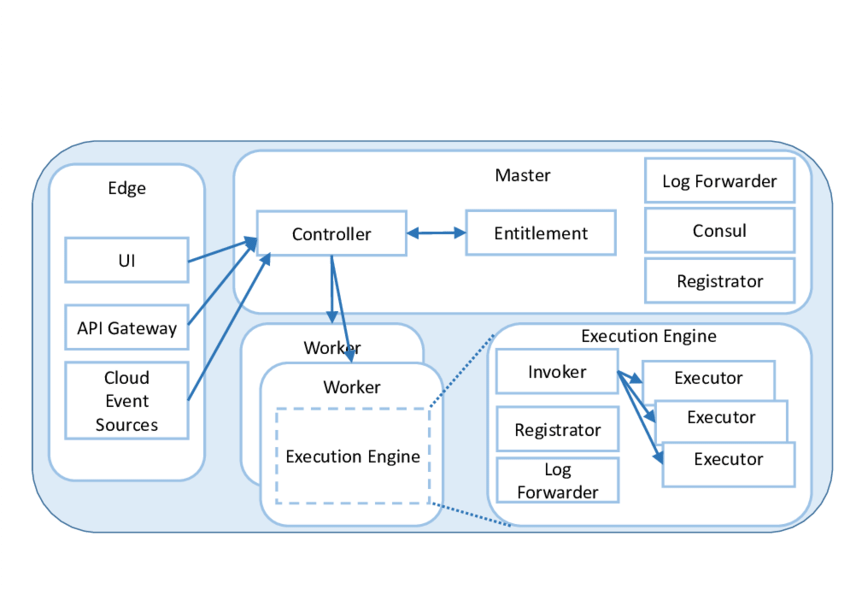
\includegraphics[width=0.9\textwidth]{baldini17-openwhisk-architecture.png}
  \caption{IBM OpenWhisk architecture \parencite{baldini17currentTrends}}
  \label{fig:openwhisk}
\end{figure}

The big four serverless platforms are compared in a recent benchmark by \textcite{malawski18benchmark}. Each platform requires the user to configure a function's memory size allocation -- apart from Azure Functions which allocate memory automatically. Available memory sizes range from 128 to 2048MB, with the per-invocation cost increasing in proportion to memory size. Measuring the execution time of CPU-intensive workloads with varying function sizes, the authors observe interesting differences in resource allocation between the different providers. AWS Lambda performs fairly consistently with CPU allocation increasing together with memory size as per the documentation. Google Cloud Functions instead behave less predictably with the smallest 128MB functions occasionally reaching the performance of the largest 2048MB functions. The authors suggest that this results from an optimization in container reuse, since reusing already spawned faster instances is cheaper than spinning up new smaller instances. Azure Functions show on average slower execution times, which the authors attribute to the underlying Windows OS and virtualization layer. On both Azure Functions and IBM Bluemix performance does not depend on function size.

\textcite{wang18peekingbehindcurtains} ``conduct the largest measurement study to date, launching more than 50,000 function instances across these three services, in order to characterize their architectures, performance, and resource management efficiency''.

\section{Security} \label{sec:security}

Similarly to PaaS, serverless architecture addresses most of the OS-level security concerns by pushing infrastructure management to the provider. Instead of users maintaining their own servers, security-related tasks like vulnerability patching, firewall configuration and intrusion detection are centralized, which has the benefit of reducing the attack surface. On the provider side the key issue becomes guaranteeing isolation between functions, as arbitrary code from many users is running on the same shared resources \parencite{mcgrath17implement}. Since strong isolation has the downside of longer container startup times, the problem becomes finding an ideal trade-off between security and performance. \parencite{van2017spec}

In case of the BaaS model, the main security implication is greater dependency to third party services \parencite{segal18risks}. Each BaaS component represents a potential point of compromise, so it becomes important to secure communications, validate inputs and outputs and minimize and anonymize the data sent to the service. \textcite{robert2016serverlessarchitectures} also notes that since BaaS components are used directly from the clients there's no protective server-side application in the middle, which requires significant care in designing the client application.

The FaaS model has a couple of advantages concerning security. First, FaaS applications are more resistant towards Denial of Service (DoS) attacks due to the platform's near limitless scalability -- although such an attack can still inflate the monthly bill and inflict unwanted costs. Second, compromised servers are less of an issue in FaaS since functions run in short-lived containers that are repeatedly destroyed and reset. Overall, as put by \textit{wagner16resilient}, ``there is a much smaller attack surface when executing on a platform that does not allow you to open ports, run multiple applications, and that is not online all of the time''. On the other hand application-level vulnerabilities remain as much of an issue in FaaS as in conventional cloud platforms. The architecture has no inherent protection against SQL injection or XSS and CSRF attacks, so existing mitigation techniques are still necessary. Vulnerabilities in application dependencies are another potential threat, since open-source libraries often make up the majority of the code in actual deployed functions. Also, the ease and low cost of deploying a high number of functions, while good for productivity, requires new approaches to security monitoring. With each function expanding the application's attack surface it's important to keep track of ownership and allocate a function only the minimum privileges needed to perform the intended logic. Managing secure configuration per each funtion can become cumbersome with fine-grained applications consisting of dozens or hundreds of functions. \parencite{podjarny17security}

A study by the security company PureSec lists a number of prominent security risks specific to serverless architectures \parencite{segal18risks}. One potential risk concerns event data injection, i.e. functions inadvertently executing malicious input injected among the event payload. Since serverless functions accept a rich set of event sources and payloads in various message formats, there are many opportunities for this kind of injection. Another risk listed in the study is execution flow manipulation. Serverless architectures are particularly vulnerable to flow manipulation as serverless applications typically consist of many discrete functions chained together in a specific order. Application design might assume that a function is only invoked under specific conditions and only by authorized invokers. For example a function might forego a sanity check on the assumption that such a check has already been passed in some previous step. By manipulating execution order an attacker might be able to sidestep access control and gain unwanted entry to some resource.
Overall the study stresses that since serverless is a new architecture its security implications are not yet well understood. Likewise security tooling and practices still lack in maturity.

\section{Economics of serverless} \label{sec:economics}

\textcite{eivy2017wary} and \textcite{villamizar2016infrastructure} both focus on the economic aspects of serverless. \textcite{adzic2017serverless} explain how novel design patterns are used to significantly optimize costs -- just running traditional web apps inside Lambda containers doesn't necessarily equate to savings. \textcite{adzic2017serverless} also report savings between 66 and 95\% in two case studies, and present a handly table comparing hosting prices for intermittent service tasks. \textcite{spillner17exploiting} exploits the control plane of AWS Lambda to implement services practically for free. \textcite{leitner16modelcost} present an approach to model deployment costs of AWS Lambda applications in real-time. \textcite{kuhlenkamp17costradamus} present another cost-tracing system that enables per-request cost-tracing for cloud-based software services, noting that cost testing should not only rely on isolated tests of single services but consider comprehensive end-to-end cost traces. \textcite{albuquerque17faaspaas} have a detailed price comparison running the same app in FaaS and PaaS. \textcite{wagner16resilient} argue that ``managed code execution services such as AWS Lambda and GCP’s Google Cloud Functions can significantly reduce the cost of operating a resilient system even in comparison to spot and preemptible VMs''. The benchmark by \textcite{malawski18benchmark} show that small functions run on faster resources on Google's platform.

The basic serverless pricing models follow a pay-per-use paradigm. As reported by \textcite{lane13baas} in a survey on the BaaS space, the most common pricing models offered by BaaS providers are billing on either the number of API calls or the amount of cloud storage consumed. The popularity of these pricing models reflects on the other hand the central role of API resources in BaaS as well as the fact that storage forms the biggest cost for BaaS providers. Beyond API call and storage pricing there are also numerous other pricing models to account for the multitude of BaaS types. Among the surveyed BaaS providers some charge per active user or consumed bandwidth, whereas others charge for extra features like analytics and tech support.

Pricing among FaaS providers is more homogeneous. FaaS providers typically charge users by the combination of number of invocations and their execution duration. Execution duration is counted in 100ms increments and rounded upwards, with the 100ms unit price depending on the selected function size. Each parallel function execution is billed separately. For example at the time of writing in AWS Lambda the price per invocation is \$0.0000002 and computation is priced at \$0.00001667 per GB-second \parencite{awslambda0218}. The unit of GB-second refers to 1 second on execution time with 1GB of memory provisioned. Given this price per GB-second, the price for 100ms of execution ranges from \$0.000000208 for 128MB functions to \$0.000004897 for 3008MB functions. At this price point, running a 300ms execution on a 128MB function 10 million times would add up to about \$8.25. The other major providers operate roughly at the same price point \parencite{microsoft18azureFunctions,ibm18cloudFunctions,google18cloudFunctions}. Most providers also offer a free tier of a certain amount of free computation each month. The AWS Lambda free tier for example includes 1 million invocations and 400,000 GB-seconds (which adds up to 800,000 seconds on the 512MB function, for example) of computation per month.

\textcite{villamizar2016infrastructure} present an experiment comparing the cost of developing and deploying the same web application using three different architecture and deployment models: monolithic architecture, microservices operated by the cloud customer, and microservices operated by the cloud provider i.e. FaaS. The results come out in favor of FaaS, with more than a 50\% cost reduction compared to self-operated microservices and up to a 77\% reduction in operation costs compared to the monolithic implementation. The authors note however that for applications with small numbers of users, the monolithic approach can be a more practical and faster way to start since the adoption of more granular architectures demands new guidelines and practices both in development work and in an organizational level. Looking only at infrastructure costs, FaaS emerges as the most competetive approach.

To demonstrate how FaaS pricing works out in the customer's advantage in the case of intermittent computation, \textcite{adzic2017serverless} compare the cost of running a 200ms service task every 5 minutes on various hosting platforms. Running a 512MB VM with an additional fail-over costs \$0.0059 per hour, whereas a similarly sized Lambda function executing the described service task costs \$0.000020016 for one hour -- a cost reduction of more than 99.8\%. The authors also present two real-world cases of FaaS migration. The first case, a mind-mapping web application, was migrated from PaaS to FaaS and resulted in hosting cost savings of about 66\%. In the second case a social networking company migrated parts of their backend services from self-operated VMs to FaaS, and estimated a 95\% reduction in operational costs.

TODO other real-world cases

A large part of the expenses incurred in developing today's computer systems derive from the need for \textit{resiliency}. Resiliency means the ability to withstand a major disruption caused by unknown events. A resilient system is expected to be up and functioning at all times, while simultaneously providing good performance and certain security guarantees. Meeting these requirements forces organizations to over-provision and isolate their cloud resources which leads to increased costs. The FaaS model can significantly reduce the cost of resiliency by offloading resource management to the provider. This was exemplified in the above uses cases, where majority of the cost savings arose from not having to pay for excess or idling resources. \parencite{wagner16resilient}

a big part of provider income comes from auxiliary services \parencite{fox17}

however eivy
not quite there yet as observed by \textcite{fox17}, since network waiting time is wasted

\section{Drawbacks and limitations} \label{sec:limitations}

What to take into consideration when migrating to serverless?

\textcite{lloydserverless} analyze serverless performance and elasticity, identifying the cold start phenomenon. Differences in runtimes/languages, and larger library dependencies lead to slower starts. \textcite{oakes17pipsqueak} address the problem by caching package dependencies on platform-level. \textcite{boucher18puttingmicroback} identify latency as an important problem (``a microservice is only as fast as the slowest service it relies on'') and introduce restructuring of FaaS architecture centered around low-latency.

\textcite{baldini17trilemma} identify three competing constraints in serverless function composition: functions should be considered as black boxes; function composition should obey a substitution principle with respect to synchronous invocation; and invocations should not be double-billed.

\textcite{robert2016serverlessarchitectures}, \textcite{adzic2017serverless} and \textcite{baldini17currentTrends} each list a number of limitations, including lack of strong SLA, vendor lock-in, short life-span, immature local development tools, statelessness and many others.

\textcite{kuhlenkamp17costradamus} discover two serverless cost tradeoffs: the retry cost effect and the cost ripple effect.

\textcite{malawski18benchmark} talk about interoperability challenges running a heterogeneous benchmark, as well as discussion on RAM allocation.

\textcite{cncf18serverlessWG} on technical immaturity, lack of interoperability, standardization, tools, documentation, best practices.

\textcite{eivy2017wary} notes that function size choosing is in fact paying for allocation, not the ``pay what you use''-promise of serverless. \textcite{microsoft18azureFunctions} has automatic memory provisioning.

The need for circuit breakers (risk of DDoSing yourself) when interacting with non-serverless components like a database. Mention novel cloud-native database services like Google's Cloud Spanner and AWS Aurora. Figure out a source for this -- \textcite{hohpe2004enterprise} might have a relevant pattern.

Address maintainability: debugging serverless functions, following the flow of control can be tough.

Composing serverless functions is not like composing regular functions. All the difficulties of distributed computing -- message loss, timeouts and others -- apply and have to be handled. Possible solutions include retry policies, dead-letter queues and idempotent functions.

A full-fledged general-purpose serverless computing model is still a vision that needs to be achieved. \parencite{buyya2017manifesto}

Unlike the abstract concept of cloud functions, FaaS cannot completely abstract away all operation logic from the user. The FaaS user can still change parameters and configurations, such as the suggested memory size or number of CPUs of the underlying function host, which influence the operation of the deployed cloufunction. \parencite{van2017spec}

AWS whitepaper \parencite{aws18architectures} lists best practices.

\textcite{van18perfchallenges} identify 6 performance-related challenges for the serverless domain and plot a roadmap for alleviating these challenges.

\textcite{leitner18industrialpractice} find that building serverless applications requires a ``different mental model that emphasizes plugging together small microservices''.

\chapter{Serverless design patterns} \label{cha:patterns}

In this chapter we take a look at serverless design patterns. Design patterns describe commonly accepted, reusable solutions to recurring problems \parencite{hohpe2004enterprise}. A design pattern is not a one-size-fits-all solution directly translatable into software code, but rather a formalized best practice that presents a common problem in its context along a general arrangement of elements that solves it \parencite{gamma94designPatterns}. The patterns in this chapter are sourced from scientific literature on serverless computing as well as cloud provider documentation \parencite[][]{aws18serverlessLens, microsoft18cloudPatterns}. Literature on object-oriented patterns (OOP) \parencite{gamma94designPatterns}, SOA patterns \parencite{rotem12soa} as well as enterprise integration patterns (EIP) \parencite{hohpe2004enterprise} was also reviewed for applicable practices.

TODO Enterprise integration patterns (EIP), as serverless is all about integrations. \textcite{hohpe2004enterprise} present a number of asynchronous messaging architectures in the seminal book on EIP. While predating the whole serverless phenomenon the patterns are still relevant. Hohpe even demonstrated implementing one of his patterns on top of Google's serverless platform \href{http://www.enterpriseintegrationpatterns.com/ramblings/google_cloud_functions.html}{in a blog post}. E.g. patterns like Idempotent Receiver, Dead-letter Channel as well as the 4 more general integration styles of File Transfer, Shared Database, RPC and Messaging. Many patterns implemented internally by FaaS platforms already!

TODO SOA patterns: as FaaS functions are self-contained nanoservices these might have some relevance. SOA patterns \parencite{rotem12soa} include Saga, Decoupled Invocation and others. As with EIP, some patterns are already implemented by the FaaS platform.

TODO FaaSification: \textcite{spillner17transformpython} describes an automated approach to transform monolithic Python code into modular FaaS units by partially automated decomposition. Doesn't really seem suitable for the web application migration process covered in this thesis but worth mentioning.

\section{Composition patterns} \label{sec:compositionPatterns}

The following patterns concern serverless function composition: how to compose and orchestrate serverless functions together into more extensive sequences or workflows?

\subsection{Routing Function} \label{subsec:routingFunction}

\textbf{Problem:} How to branch out execution flow based on request payload?

\begin{figure}[h]
  \centering
  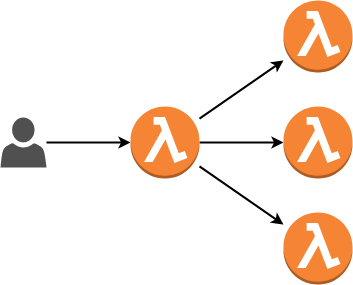
\includegraphics[width=0.4\textwidth]{patterns/routing-function.png}
  \caption{Routing Function}
  \label{fig:patternRoutingFunction}
\end{figure}

\textbf{Solution:} Use a central routing function to receive requests and invoke appropriate functions based on request payload.

This pattern involves instantiating a routing function that contains all the necessary information to route requests to other functions. All function invocations are directed to the routing function, which in turn invokes target functions according to request payload. The routing function finally passes target function return value over to the client.

It's notable that FaaS platforms commonly provide API gateways and other tools for routing, for example the Amazon API Gateway \parencite{awslambda0218}. These tools however are mostly limited to path-based routing, whereas a routing function can be implemented to support more dynamic use cases. Also interestingly, according to an industry survey \parencite{leitner18industrialpractice}, some practicioners opted for the Routing Function pattern over platform API gateway services as they found the latter cumbersome to manage. \textcite{sbarski2017serverless} similarly postulate that the pattern ``can simplify the API Gateway implementation, because you may not want or need to create a RESTful URI for every type of request''. Another advantage of the pattern is that the routing function can be used to supplement request payload with additional context or metadata. A centralized routing function also means that all routing configuration is found in one place, and that public-facing API routes only need to be configured for one function, not all of them \parencite{leitner18industrialpractice}. From a service client's point of view, the Routing Function has the benefit of abstracting backend services so that calls can be rerouted to different services without changing client implementation; this can be put to use for example in A/B testing by partially rolling out new updates to selected clients \parencite{microsoft18cloudPatterns}.

The pattern's major disadvantage is double billing, as the routing function essentially has to block and wait until the target function finishes execution. Additionally, as routing is implemented at function code level, information about function control flow gets hidden in implementation rather than being accessible from configuration \parencite{leitner18industrialpractice}. Also, akin to any centralized service, the Routing Function can potentially introduce a single point of failure or a performance bottleneck \parencite{microsoft18cloudPatterns}.

The Routing Function resembles the OOP Command pattern, which is used to decouple caller of the operation from the entity that carries out the processing via an intermediary command object \parencite{gamma94designPatterns}. A related EIP pattern is the Content-Based Router, which ``examines the message content and routes the message onto a different channel based on data contained in the message'' \parencite{hohpe2004enterprise}. Also pertinent to the serverless Routing Function, \textcite{hohpe2004enterprise} caution that the Content-Based Router should be made easy to maintain as it can become a point of frequent configuration. Finally, Microsoft's cloud design patterns includes the Gateway Routing pattern that's similarly employed to ``route requests to multiple services using a single endpoint'' \parencite{microsoft18cloudPatterns}.

\subsection{Function Chain} \label{subsec:functionChain}

\textbf{Problem:} Task exceeds maximum function execution duration, resulting in a timeout.

\begin{figure}[h]
  \centering
  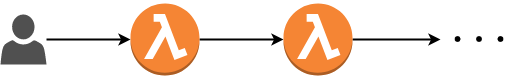
\includegraphics[width=0.5\textwidth]{patterns/function-chain.png}
  \caption{Function Chain}
  \label{fig:patternFunctionChain}
\end{figure}

\textbf{Solution:} Split the task into separate function invocations that are chained together sequentially.

The Function Chain comprises of an initial function and any number of subsequent functions. The initial function begins computation while keeping track of remaining execution time. Foe example in AWS Lambda the execution context contains information on how many milliseconds are left before termination \parencite{awslambda0218}. Upon reaching its duration limit, the initial function invokes another function asynchronously, passing along as parameters any state necessary to continue task computation. Since the intermediary invocation is asynchronous (``fire-and-forget''), the initial function can terminate without affecting the next function in chain.

The Function Chain pattern is in effect a workaround over the duration limit that FaaS platforms place on function execution \parencite{leitner18industrialpractice}. The pattern was reported to be used at least occasionally in an industry study by \textcite{leitner18industrialpractice}. Its disadvantages include strong coupling between chained functions, increase in the number of deployment units and the overhead of transferring intermediate execution state and parameters between each chained function. \textcite{leitner18industrialpractice} also note that splitting some types of tasks into multiple functions can be difficult. Finally, as the pattern relies on asynchronous invocation, the last function in chain has to persist computation result into an external storage for the client to access it, which brings in further dependencies.

\subsection{Fan-out/Fan-in} \label{subsec:FanoutFanin}

\textbf{Problem:} Resource limits on a single function lead to reduced throughput.

% TODO visualize
% \begin{figure}[h]
%   \centering
%   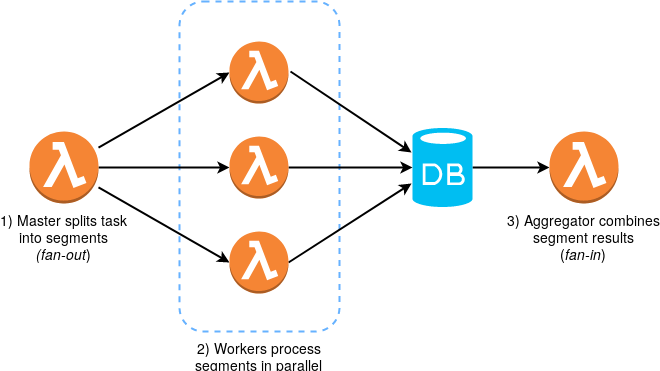
\includegraphics[width=0.4\textwidth]{patterns/fan-out-fan-in.png}
%   \caption{Fan-out/Fan-in}
%   \label{fig:fantOutFanIn}
% \end{figure}

\textbf{Solution:} Split task into multiple parallel invocations.

As discussed, serverless functions are limited in execution duration as well as CPU and memory capacity. The Function Chain pattern (section \ref{subsec:functionChain}) works around the former limitation but is still constrained by a single function's computing resources, which can result in prohibitively slow throughput for compute-intensive tasks. The Fan-out/Fan-in pattern is an alternative approach that takes advantage of serverless platforms' inherent parallelism. The pattern consists of a master function that splits the processing task into segments and then asynchronously invokes a worker function for each segment. Having finished processing, each worker function stores its result on a persistence layer, and finally an aggregator function combines the worker results into a single output value -- although the aggregation step can be omitted in cases where intermediary results suffice. As each worker function invocation runs in parallel with its own set of resources, the pattern leads to faster completion of the overall task. \parencite{zambrano18patterns}

The Fan-out/Fan-in pattern lends itself well to tasks that are easily divisible into independent parts: the efficiency gained depends on the granularity of each subdivision. Conversely, an apparent limitation to the pattern is that not all tasks can be easily distributed into separate worker functions. \textcite{mcgrath16cloudEventParadigms} utilize the pattern in ``easily and performantly solving a large-scale image resizing task''. The authors point out how the pattern reduces development and infrastructure costs compared to a traditional multi-threaded application which ``typically demands the implementation of a queueing mechanism or some form of worker pool''. \textcite{lavoie19efficiency} similarly study ``the efficiency of a serverless architecture for running highly parallelizable tasks'' in comparison to a conventional MapReduce solution running on Apache Spark, concluding that ``the serverless technique achieves comparable performance in terms of compute time and cost''.

\textcite{hohpe2004enterprise} present a similar approach to messaging with the EIP pattern of Composed Message Processor, which ``splits the message up, routes the sub-messages to the appropriate destinations and re-aggregates the responses back into a single message.''

\subsection{State Machine} \label{subsec:stateMachine}

\textbf{Problem:} How to coordinate complex, stateful procedures with branching steps?

\begin{figure}[h]
  \centering
  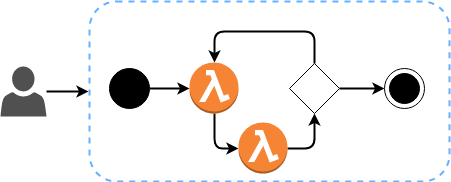
\includegraphics[width=0.6\textwidth]{patterns/state-machine.png}
  \caption{State Machine}
  \label{fig:patternStateMachine}
\end{figure}

\textbf{Solution:} Split a task into a number of discrete functions and coordinate their execution with an orchestration tool.

\textcite{hong18securingviaserverlesspatterns} describe the State Machine pattern as ``building a complex, stateful procedure by coordinating a collection of discrete Lambda functions using a tool such as AWS Step Functions''. These orchestration tools consist of a collection of workflow states and transitions between them, with each state having its associated function and event sources -- essentially a serverless a state machine \parencite{cncf18serverlessWG}. Figure \ref{fig:patternStateMachine} could for example represent a workflow where the first function attempts a database insert, the second function checks whether the operation succeeded, and depending on the result either the operation is retried or execution is finished. The advantage of using provider tooling for workflow execution is that there's no need for external storage as the orchestrator keeps track of workflow state. Downsides on the other hand include extra cost arising from orchestration tooling as well as the overhead of managing workflow descriptions.

\textcite{lopez18orchestration} compare three major FaaS orchestration systems: AWS Step Functions, IBM Composer and Azure Durable Functions. The compared systems typically support function chaining, conditional branching, retries and parallel execution, with workflows defined either in a Domain-Specific Language or directly in code. One restriction in Amazon's orchestrator is that a composition cannot be synchronously invoked and is thus not composable in itself: a state machine cannot contain another state machine. AWS Step Functions was also the least programmable among the compared systems, but on the other hand the most mature and performant. Finally, the authors observe that none of the provider-managed orchestration systems are prepared for parallel programming, with considerable overheads in concurrent invocation.

A SOA pattern analogous to serverless orchestration tools is the Orchestrator, in which ``an external workflow engine activates a sequence (simple or compound) of services to provide a complete business service''. The Orchestrator aims to keep business processes agile and adaptable by externalizing them from service implementations: instead of hard-coding service interactions they are defined, edited and executed within a workflow engine. Used properly, the Orchestrator can add a lot of flexibility to the system. Difficulty however lies in implementing services as composable and reusable workflow steps while still keeping them useful as autonomous services. \parencite{rotem12soa}.

\subsection{Thick Client} \label{subsec:thickClient}

\textbf{Problem:} How to coordinate access to third party cloud services while avoiding extra costs?

\begin{figure}[h]
  \centering
  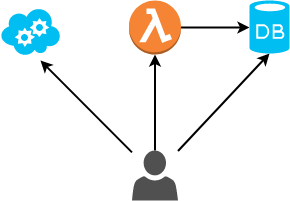
\includegraphics[width=0.5\textwidth]{patterns/thick-client.png}
  \caption{Thick Client}
  \label{fig:patternThickClient}
\end{figure}

\textbf{Solution:} Create thicker, more powerful clients.

Serverless applications, as described in chapter \ref{cha:serverless}, typically rely heavily on third party cloud services (BaaS) interspersed with custom logic in form of serverless functions. In a traditional three-tier web application architecture interaction with these external services would be handled by a server application that sits between the client and the service layers \parencite{robert2016serverlessarchitectures}. Following this model, the client can be limited in functionality whereas the server application plays a larger role. \textcite{sbarski2017serverless} point out that the model of the backend as a gatekeeper between client and services is in conflict with the serverless paradigm. First of all, using FaaS as a middle layer in front of cloud resources directly translates into extra costs: on top of paying for the cloud service call, one has to pay for function invocation and execution for the duration of the network call as well as data transfer between the service and the FaaS provider. Secondly, a middle layer of FaaS results into extra network hops which increases latency and reduces user experience. \textcite{sbarski2017serverless} thus advise against routing everything through a FaaS layer, and advocate building thick clients that communicate directly with cloud services and orchestrate workflows between them.

In addition to the cost benefit, a Thick Client has the advantage of improved changeability and separation of concerns, as the single monolithic backend application is replaced by isolated and self-contained components. Doing away with the central arbiter of a server application does come with its trade-offs, including a need for distributed monitoring and further reliance on the security of the cloud services. Importantly not all functionality can or should be moved to the client: security, performance or consistency requirements among others can necessitate a server-side implementation. \parencite{robert2016serverlessarchitectures}.

The Thick Client pattern depends on fine-grained, distributed, request-level authentication in lieu of a gatekeeper server application. This follows naturally from the way serverless functions operate: being stateless and continuously scaling up and down, maintaining a session between the backend and the cloud services is infeasible. Instead of automatically trusting all requests originating from the backend, each cloud service request has to be individually authorized. From a cloud service's point of view, requests originating from a serverless function or directly from the client are both equally untrusted. Hence in serverless architectures, skipping the backend layer is preferable whenever a direct connection between client and services is possible. The Valet Key pattern in section \ref{subsec:valetKey} describes one example of a request-level authentication mechanism. \parencite{adzic2017serverless}

\section{Event patterns} \label{sec:eventPatterns}

Event patterns deal with workflows that are triggered by external events and processed on-demand and asynchronously. FaaS platforms are a good fit for event-driven workflows as they offer integrations to a wide range of event sources as well as non-blocking invocation methods.

\subsection{Event Processor} \label{subsec:Eventprocessing}

\textbf{Problem:} How to execute a task on-demand upon event occurrence?

\begin{figure}[h]
  \centering
  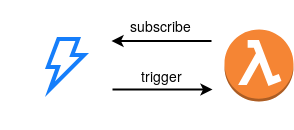
\includegraphics[width=0.45\textwidth]{patterns/event-processor2.png}
  \caption{Event Processor}
  \label{fig:patternEventProcessor}
\end{figure}

\textbf{Solution:} Subscribe a serverless function to a cloud event such as file upload or database change.

The Event Processor pattern consists of subscribing a serverless function to a cloud event source so that when the event occurs, the subscribed function gets invoked with the event context as a parameter \parencite{hong18securingviaserverlesspatterns}. Serverless platforms typically offer a number of integration points to events that originate from various other platform services. For example AWS Lambda functions can be triggered by file uploads, database change events, message queue and notification services, IoT events and others \parencite{awslambda0218}.

\textcite{baldini17currentTrends} mention thumbnail generation triggered by image upload as an exemplary use case of serverless event processing: a bursty, compute-intensive task triggered on-demand by a cloud event. A traditional approach would be to implement a poller system that regularly checks for new images and generates thumbnails as images are detected. Such a system would require constant operation, and depending on polling interval the design leads to either extra network traffic or potentially long delay between event occurrence and processing. The design is especially wasteful in cases where new images come in infrequently. The Event Processor pattern, in turn, can bring considerable cost benefit in case of infrequent or irregular workflows as computation is only ran when necessary \parencite{hong18securingviaserverlesspatterns}. Another advantage is scalability, as functions are automatically invoked as per the number of events: a large number of events occurring at once leads to a similarly large number of serverless functions executing in parallel \parencite{hong18securingviaserverlesspatterns}.

The Event Processor has two counterparts among SOA patterns. In terms of scalability, a serverless Event Processor essentially implements the Service Instance pattern which involves ``deploying multiple instances of service business logic'' to address increased service load. Aptly, the Service Instance pattern is ``best suited for stateless service implementations''. Another related SOA pattern is the Inversion of Communications in which services eschew point-to-point communication in favour of event-driven architecture to reduce coupling between event sources and consumers. The pattern's downsides include the added complexity of designing a system as events and the difficulty of debugging complex event chains. \parencite{rotem12soa}

The Event Processor can also be seen as a serverless form of the Event-Driven Consumer EIP pattern: a message consumer that sits dormant with no active threads until invoked by the messaging system. In essence, the pattern bridges the gap between external events and application-specific callbacks. A notable feature of an Event-Driven Consumer is that it automatically consumes messages as soon as they become available, which in effect means that the consumer has no control on its consumption rate: see the Polling Event Processor in section \ref{subsec:PollingEventProcessor} for an alternative solution. \parencite{hohpe2004enterprise}

Another point to keep in mind when implementing the Event Processor pattern is that some cloud event sources operate in at-least-once message delivery semantics: due to the highly distributed and eventually consistent nature of cloud platforms, events are guaranteed to be triggered at least once, not exactly once \parencite{awslambda0218}. This means that the triggered serverless function should in effect act idempotently, i.e. multiple executions with the same context should result in identical side effects. \textcite{hohpe2004enterprise} introduce a similar concept with the Idempotent Receiver pattern, a listener that can ``safely receive the same message multiple times''. The authors introduce two primary means for achieving idempotency: either explicit deduplication at the receiving end, or defining message semantics to support idempotency. The first approach calls for keeping track of the messages received thus far and ignoring any duplicates among incoming messages, leaving us with the problem of where and for how long to store the message history. The alternative approach is to design messages themselves in a way that ``resending the message does not impact the system'': for example \textit{set account balance to \$10} instead of \textit{increase account balance by \$1}.

\subsection{Periodic Invoker} \label{subsec:periodicInvocation}

\textbf{Problem:} How to execute a task periodically in predefined intervals?

\begin{figure}[h]
  \centering
  
\includegraphics[width=0.4\textwidth]{patterns/periodic-invocation.png}
  \caption{Periodic Invoker}
  \label{fig:patternPeriodicInvocation}
\end{figure}

\textbf{Solution:} Subscribe a serverless function to a scheduler.

This pattern represents an arrangement where a serverless function is invoked periodically by a scheduler, akin to a cron task in Unix-based systems. First, the scheduler invokes the subscribed function according to its configuration. Second, the function carries out its task. Finally, after execution the function can report execution result out to a notification channel, store it in database or shut down if we're not interested in the outcome. The pattern is both conceptually simple and easy to implement, as all the major serverless providers offer integration to a cloud-based scheduler such as AWS CloudWatch Events \parencite{awslambda0218}. Potential use cases include periodical backups, compliance checks, service health checks, database cleanup tasks and other background jobs that are not latency-critical. \parencite{hong18securingviaserverlesspatterns}

\subsection{Polling Event Processor} \label{subsec:PollingEventProcessor}

\textbf{Problem:} How to react to a state change in an external service that doesn't offer an event source?

\begin{figure}[h]
  \centering
  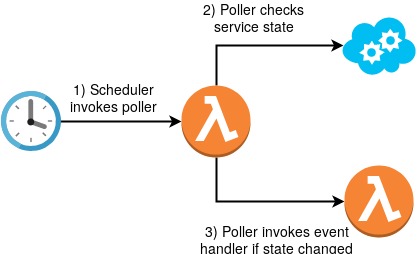
\includegraphics[width=0.4\textwidth]{patterns/polling-event-processor.png}
  \caption{Polling Event Processor}
  \label{fig:PollingEventProcessor}
\end{figure}

\textbf{Solution:} Use the Periodic Invoker pattern to create a polling event processor.

The Event Processor pattern (section \ref{subsec:Eventprocessing}) is used to perform a task in reaction to some state change in another system. The pattern depends on the external system to actively invoke the subscribed function when said state change occurs. Not all systems however are capable of performing such callbacks on state changes, which renders the pattern infeasible in some cases. To work around this limitation we can combine the Event Processor and Periodic Invoker patterns (section \ref{subsec:periodicInvocation}) to essentially implement an event-driven integration point in front of a service where no such event source originally exists. The Polling Event Consumer pattern consists of a Periodic Invoker that repeatedly checks the state of another service and performs a task when found state matches some condition. The task performed can be either implemented in the polling function itself or separated to another function that the poller invokes.

The Polling Event Processor is equivalent to the EIP pattern of Polling Consumer, where a receiver synchronously polls for a message, processes it and then polls for another. As well as offering eventful integration to non-eventful services, the pattern has the advantage of controlling its consumption rate. Whereas the Event Processor executes tasks as soon as events occur, the Polling Event Processor explicitly polls for new events when it is ready for them. The polling interval can also be configured to implement batching. As a downside, a sparse polling interval leads to increased latency between event occurrence and task execution. On the other hand a more fine-grained polling interval results in wasted resources when there are no events to consume. In short, ``polling enables the client to control the rate of consumption, but wastes resources when there’s nothing to consume.'' \parencite{hohpe2004enterprise}

\subsection{Event Broadcast} \label{subsec:EventBroadcast}

\textbf{Problem:} How to invoke multiple parallel functions as a result of a single event occurrence?

% TODO visualize
% \begin{figure}[h]
%   \centering
%   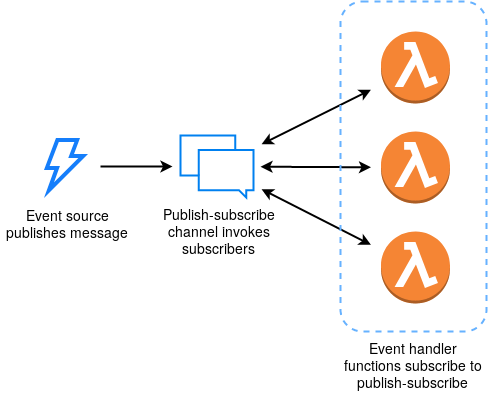
\includegraphics[width=0.4\textwidth]{patterns/event-broadcast.png}
%   \caption{Event Broadcast}
%   \label{fig:eventBroadcast}
% \end{figure}

\textbf{Solution:} Subscribe multiple functions to a notification service, publish notification on event occurrence.

The Event Processor pattern \ref{subsec:Eventprocessing} is applicable within cases of a 1-to-1 relationship between events and tasks, as exemplified above with image upload triggering thumbnail generation. However in other cases a single event can result in multiple independent tasks. For example the image upload event could as well trigger a database update and a notification email, adding up to three self-contained and parallel tasks. Most event sources only support invoking one function per event which leaves us with a couple of options. First, we could set up a new function that subscribes to the image upload event and in turn asynchronously invokes any number of processor functions, as a sort of a parallel Routing Function \label{subsec:routingFunction}. This approach comes with the operational overhead of needing to set up and maintain an additional function per each event broadcast. An alternative solution is to utilize a publish-subscribe channel such as the AWS Simple Notification Service \parencite{awslambda0218}. The key feature of a publish-subscribe channel is that any number of listeners can subscribe to a single channel, which can be used to overcome the 1-to-1 relationship between event sources and functions. Now instead of subscribing a function directly to an event source, functions subscribe to a message channel that the event source publishes a message to upon event occurrence. In addition to achieving parallel fan-out to multiple functions, the pattern has the added benefit of loosed coupling between event sources and handler functions. \parencite{sbarski2017serverless}

The Event Broadcast is derived from the Publish-Subscribe Channel EIP pattern \parencite{hohpe2004enterprise} and the Observer OOP pattern \parencite{gamma94designPatterns}. % TODO expand on this

\section{API patterns} \label{sec:apiPatterns}

Integrating with external systems.
TODO elaborate, rename to integration patterns?

\subsection{Aggregator} \label{subsec:aggregator}

\textbf{Problem:} A client must make multiple API requests to perform an operation.

TODO visualize
% \begin{figure}[h]
%   \centering
%   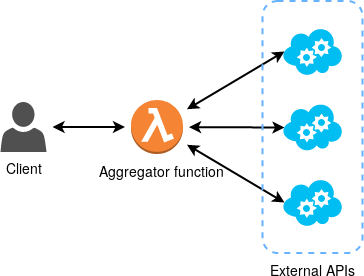
\includegraphics[width=0.4\textwidth]{patterns/aggregator.png}
%   \caption{Aggregator}
%   \label{fig:aggregator}
% \end{figure}

\textbf{Solution:} Aggregate multiple API requests under a single serverless function.

Service clients often need to deal with operations that involve performing several API calls, either in parallel or sequentially, and then filtering or combining the results. The operation might utilize multiple different services or just different endpoints of a single service. \textcite{baldini17currentTrends} use the example of combining geo-location, weather and language translation APIs to render a localized weather forecast. Another example concerns a multi-step API call of first fetching an API key, then resource location, and finally performing the actual operation. Composing operations out of multiple cross-service calls is a natural outcome of service oriented architectures, but incurs the penalty of extra resource usage and network latency in clients. The problem is further magnified in microservice and serverless architectures due to the fine service granularity. \parencite{microsoft18cloudPatterns}

The Aggregator pattern consists of wrapping the required API calls into a single serverless function which is then exposed as a singular endpoint to clients. The Aggregator calls each target API and combines the results so that the client is left with a single network call, reducing the risk of network failure. Client resource usage is also reduced since any filtering or aggregation logic is offloaded to the Aggregator. Also ideally the Aggregator function is located near backend services to minimize network latency, and individual API responses are cached whenever possible. \parencite{baldini17currentTrends}

The Aggregator is largely equivalent to the Gateway Aggregation cloud design pattern \parencite{microsoft18cloudPatterns}. \textcite{baldini17currentTrends} in turn split the pattern into API composition and API aggregation, for combined and sequential request flows respectively. It's worth noting that the Aggregator doesn't rid us of the problem of network failure and incomplete requests, as the aggregating function might still encounter failed requests from downstream services. The pattern rather outsources the risk from service consumer to a backend service, working thus opposite to the Thick Client pattern (\ref{subsec:thickClient}) where service orchestration is driven by consumers. To ensure reliable operation when one of the API requests fails the Aggregator might internally implement the Compensating Transactions cloud design pattern, i.e. pairing each request with a compensating action that is performed in case of failure \parencite{microsoft18cloudPatterns}. The SOA patterns of Transactional Service and the more heavyweight Saga could also be used to enforce transactional guarantees inside the Aggregator \parencite{rotem12soa}.

% \subsection{API Async} \label{subsec:apiAsync}

% Turn a synchronized API into an async one.

% Request/Reaction SOA \parencite{rotem12soa}.

\subsection{Proxy} \label{subsec:proxy}

\textbf{Problem:} How to make a legacy service easier to consume for modern clients?

TODO visualize
% \begin{figure}[h]
%   \centering
%   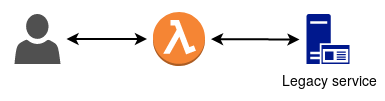
\includegraphics[width=0.4\textwidth]{patterns/proxy.png}
%   \caption{Proxy}
%   \label{fig:proxy}
% \end{figure}

\textbf{Solution:} Implement a serverless function as a proxy layer that translates requests between clients and the legacy service.

Applications often need to integrate to a legacy system for some resource or functionality. This requirement might present itself when an outdated but crucial system is in the process of being migrated, or cannot be migrated at all due to reasons of complexity or cost. Legacy systems might suffer from quality issues and use older protocols or data formats, which makes interoperation with modern clients problematic. A client would have to implement support for legacy technologies and semantics, which might adversely affect its own design goals. \parencite{microsoft18cloudPatterns}

The serverless Proxy pattern essentially ``makes legacy services easier to consume for modern clients that may not support older protocols and data formats'' \parencite{sbarski2017serverless}. The pattern consists of a serverless function that acts as a proxy in front of the legacy service, handling any necessary protocol or data format translation and sanity checks. Conversely for client applications, the Proxy offers a clean and modern API for easier consumption. \textcite{sbarski2017serverless} use the example of offering a JSON API in front of a SOAP service. The pattern is also referred to as the Anti-Corruption Layer, alluding to how it works to contain a system's quality issues: ``this layer translates communications between the two systems, allowing one system to remain unchanged while the other can avoid compromising its design and technological approach'' \parencite{microsoft18cloudPatterns}.

\subsection{Strangler} \label{subsec:strangler}

\textbf{Problem:} How to migrate an existing service to serverless architecture in a controlled fashion?

TODO visualize
% \begin{figure}[h]
%   \centering
%   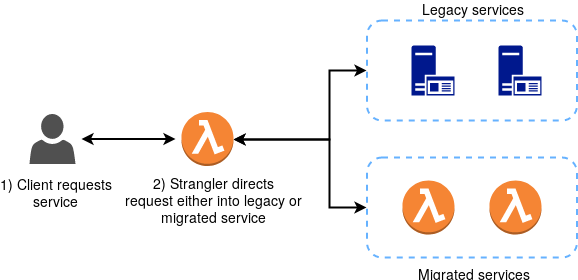
\includegraphics[width=0.4\textwidth]{patterns/strangler.png}
%   \caption{Strangler}
%   \label{fig:strangler}
% \end{figure}

\textbf{Solution:} Create a façade in front of the legacy API and incrementally replace individual routes with serverless functions.

Migrating an extensive application to serverless in one go could be a lengthy endeavour and lead to service downtime. Instead, it's often safer to perform a gradual migration where parts of an API are replaced one by one with the old system still running in the background and serving the yet to be migrated features. The problem with running two versions of the same API, however, is that clients need to update their routing every time a single feature is migrated. \parencite{microsoft18cloudPatterns}

The Strangler solves the problem of gradual migration by first wrapping the whole legacy API behind a simple façade that initially just proxies requests to the legacy API as before. Then, as individual features are migrated to serverless, the façade's internal routing is updated to point to the serverless function instead of the legacy API. Thus ``existing features can be migrated to the new system gradually, and consumers can continue using the same interface, unaware that any migration has taken place'' \parencite{microsoft18cloudPatterns}. Eventually when all features have completed migration, the old system can be phased out. \textcite{zambrano18patterns} proposes implementing the façade with an API gateway that matches and proxies all routes, but the Routing Function pattern (\ref{subsec:routingFunction}) is equally applicable here. The author also points out how the Strangler makes it easy to roll back a new implementation in case of any problems, and thus helps to reduce the risk in migration.

% \subsection{Separate FaaS handler from core logic} \label
% {subsec:separateHandler}

% Separate FaaS handler core logic in code level.

\section{Data management/access patterns} \label{sec:dataManagementPatterns}

Managing state and accessing external resources.

\subsection{Externalized State} \label{subsec:externalizedState}

\textbf{Problem:} How to share state between sequential or parallel serverless function instances?

TODO visualize
% \begin{figure}[h]
%   \centering
%   \includegraphics[width=0.4\textwidth]{patterns/externalizedState.png}
%   \caption{Externalized State}
%   \label{fig:externalizedState}
% \end{figure}

\textbf{Solution:} Store function state in external storage.

Serverless functions are, as discussed, stateless by design. Function instances are spawned and terminated ephemerally in a way that an instance has no access to any preceding or parallel instance state. Not all serverless use cases are purely stateless however, so being able to store and share state between function instances comes up as a common requirement. This is evidenced by a survey on serverless adoption in which two thirds of respondents reported at least sometimes applying the Externalized State pattern, making it by far the most common among the surveyed patterns \parencite{leitner18industrialpractice}.

The Externalized State pattern is a fundamental pattern that consists of storing a function's internal state in external storage such as a database or a key-value store. The pattern is used to reliably persist state between sequential function invocations, and on the other hand to share state between parallel invocations. Imposing state on a stateless paradigm doesn't come free though, as relying on external storage induces latency and extra programming effort as well as the operational overhead of managing a storage component. \parencite{leitner18industrialpractice}

\subsection{Valet Key} \label{subsec:valetKey}

\textbf{Problem:} How to authorize resource access without routing all traffic through a gatekeeper server process?

TODO visualize
% \begin{figure}[h]
%   \centering
%   \includegraphics[width=0.4\textwidth]{patterns/valetKey.png}
%   \caption{Valet Key}
%   \label{fig:valetKey}
% \end{figure}

\textbf{Solution:} Let the client request an access token from an authorizer function, use the token to directly access a specific resource.

As put forth in section \ref{subsec:thickClient} (the Thick Client pattern), serverless function instances do not form long-lived sessions with backend services, which means that each service request must be individually authorized. With this in mind, routing client-service requests through a serverless function brings us no apparent security advantage, as both the client and the serverless function are equally untrusted from a service's point of view; on the contrary, having an extra server layer in the middle would only introduce additional latency and cost in data transfer \parencite{adzic2017serverless}. The problem then becomes one of authorizing client-service communication without storing service credentials in the client and thus losing control of service access, and on the other hand without routing each request through the backend and thus in effect paying twice for data transfer.

The Valet Key represents one form of the fine-grained request-level authorization called for by the Thick Client pattern (\ref{fig:patternThickClient}).


avoid paying for transfer twice
relies on fine-grained authorization models in cloud services

% \subsection{Least privilege IAM role} \label{subsec:LeastprivilegeIAMrole}

% Minimize attack surface by reducing function access roles to bare minimum. Mentioned in \textcite{aws18serverlessLens}.

\section{Performance and scalability patterns} \label{sec:perfPatterns}

Address FaaS performance issues.

\subsection{Function Warmer} \label{subsec:FunctionWarmer}

Ping a function intermittently to avoid cold starts.

% \subsection{Oversized function} \label{subsec:OversizedFunction}

% Choose maximum memory allocation to access faster CPU resources and improve cold start latency.

\subsection{Singleton} \label{subsec:Singleton}

Take advantage of function execution context to avoid reinitializing function dependencies. Check \textcite{aws18serverlessLens}.

\section{Resiliency and availability patterns} \label{sec:resiliencyPatterns}

Maximize serverless system resiliency.

\subsection{Bulkhead} \label{subsec:Bulkhead}

Isolate high-latency code into separate functions to avoid resource contention.

\subsection{Flow control/throttling} \label{subsec:Flow control/throttling}

Throttle invocations to avoid DDoSing yourself. Lambda concurrency limit \textcite{aws18serverlessLens}.

\subsection{Circuit breaker} \label{subsec:Circuit breaker}

Keep track of component availability to avoid cascading failures.


\chapter{Migration process} \label{cha:migration}

This chapter describes the process of migrating a web application to serverless architecture. The goal of the process is to explore the catalogued patterns' feasibility by applying them on common problems in the domain of web application development. As well as exploring the patterns we're seeing how the distinct serverless features drive application design and trying to gain deeper understanding of the advantages and shortcomings of the paradigm. The chapter begins with the description of the migrated application along with its functional and non-functional requirements. We then identify the ways in which the current implementation fails to meet these requirements and thus set a target for the serverless implementation. Lastly a new serverless design is proposed using the pattern catalogue of Chapter \ref{cha:patterns} and in cases where the patterns prove insufficient or unsuitable, modifications or new patterns are proposed.

\section{Image Manager}

The migrated application, Image Manager, is a tool for managing image assets. Image Manager is adapted from a real-world application, although modified in places for the sake of illustration. Similarly to a SaaS offering such as Cloudinary, the application takes user-uploaded images, performs various forms of processing and then hosts and serves the processed images to be consumed by other applications. In case of Image Manager the processing needs are threefold: rendering a thumbnail, rendering a low quality image placeholder (LQIP), and automatic label detection. In short Image Manager can be split into three basic functional requirements: image upload, image processing and image hosting.

The pre-migration (or \textit{serverful}) Image Manager consists of a single server application that connects to a number of BaaS-type cloud services. These components are depicted in Figure \ref{fig:serverfulArchitecture}. The server application publishes an HTTP API endpoint for image uploads which is consumed by a browser client. In place of access control this public-facing API uses a CAPTCHA: before image upload the client requests a challenge from Google reCAPTCHA API, solves it and sends the obtained token along with the image upload request. The server application then also connects to reCAPTCHA API to verify token validity before proceeding with the upload request. A CAPTCHA is used instead of full-blown authentication to allow for anonymous users while still providing some degree of protection against bots and other illicit usage. After CAPTCHA verification the application proceeds with image processing. The thumbnail and LQIP rendering tasks are performed locally whereas labeling is handled by a network call to an external image analysis service, Google Cloud Vision API. The three processing tasks are independent and performed concurrently. Finally both the original and processed images are uploaded to Google Cloud Storage where they can be fetched via publicly accessible URLs. This image upload sequence is illustrated in further detail in Figure \ref{fig:serverfulSequence}.

\begin{figure}[H]
  \centering
  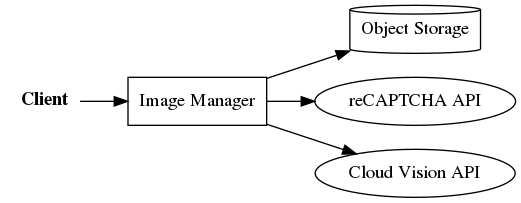
\includegraphics[width=0.65\textwidth]{image-manager.png}
  \caption{Image Manager components}
  \label{fig:serverfulArchitecture}
\end{figure}

\begin{figure}[H]
  \centering
  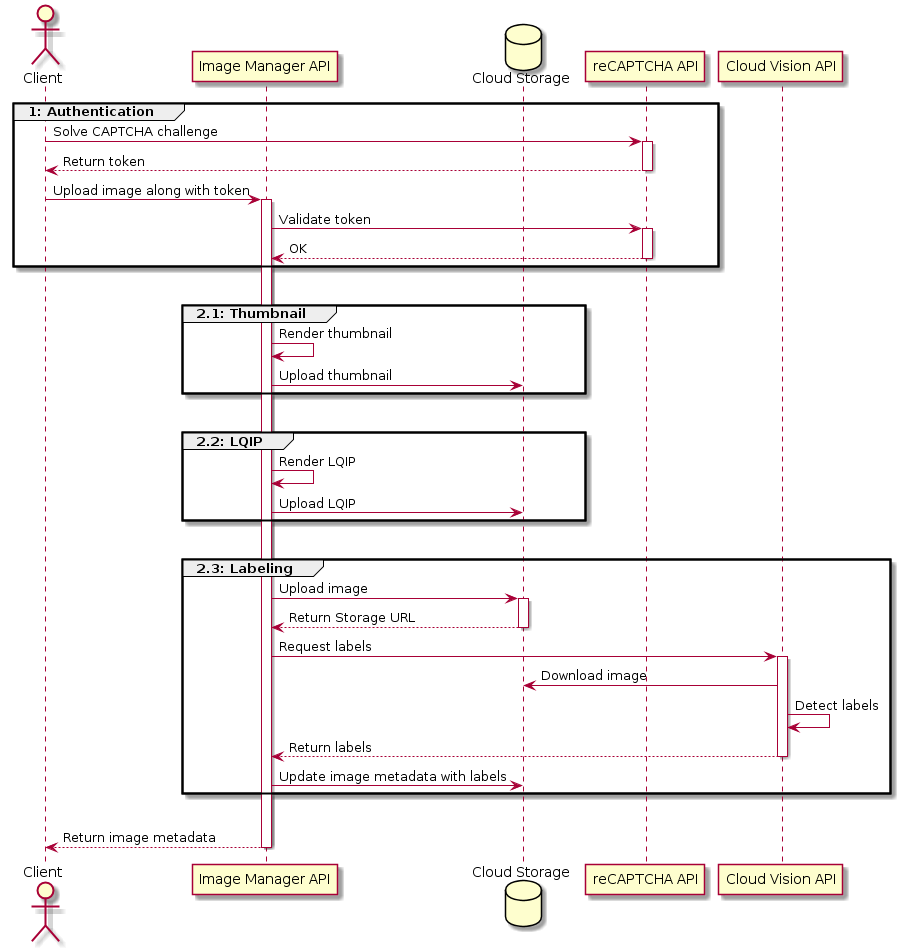
\includegraphics[width=1\textwidth]{sequence.png}
  \caption{Image Manager upload sequence}
  \label{fig:serverfulSequence}
\end{figure}

Overall the image upload task is both CPU-intensive due to rendering and I/O-heavy due to service requests and also since processing results are temporarily written on disk before cloud storage upload. As for technical details, Image Manager is written in TypeScript, transpiled into JavaScript and running on NodeJS v10. The server application is containerized into a Docker image and deployed on a single VM on Google Cloud Platform's \textit{us-east1 region}. The VM exposes an IP address through which the application is accessed from public internet.

Image Manager can even in its pre-migration state be considered \textit{cloud-ready} in the sense that it was originally designed and developed to run specifically in a cloud environment. This is reflected in the usage of container technology and the reliance on cloud platform services in favour of self-managed code. The degree of cloud-readiness should be kept in mind when considering the migration process as the practices and observations might not apply when starting off with a more conventional on-premise application architecture.

The motivation to migrate Image Manager to serverless architecture stems from a number of shortcomings in the current implementation, specifically relating to the non-functional requirements of availability, scalability, cost-efficiency and isolation. First, the obvious drawback of the server application's single-VM deployment is poor availability as there is no failover instance to take over in case of VM failure. Likewise the application's capacity to serve traffic is limited by a single VM's computing resources as there is no scaling mechanism in play. Achieving this double goal of availability and scalability, i.e. ensuring a correct number of VMs to meet current demand at all times would require a considerable amount of infrastructure configuration involving load balancing, clusterization and scaling policies \parencite{jonas19berkeleyView}. This inelasticity also results in cost-inefficiency as the VM instance is constantly running and accumulating charges whether there is any traffic or not. Lack of isolation is also a concern since all application logic is bundled together into a single monolithic application which causes resource contention as for example high CPU usage in one of the rendering tasks can divert resources from the API and result in connection timeouts. This combined with processing tasks' highly asymmetrical performance profiles also further complicates scaling as we can only scale the whole application, not just the bottlenecks. Lack of isolation also presents itself in how all traffic is routed through the server application, which in case of image uploads means an extra network trip before reaching Cloud Storage. Finally, the server application's monolithic design has negative maintainability implications since modifications cannot be developed or deployed independently.

\section{Serverless Image Manager}

Rewriting an application in serverless architecture is clearly not a trivial task nor does it have a single correct solution. Comparable to building a system out of microservices or plotting class hierarchy in object-oriented software design, the same outcome can be achieved with a variety of different but equally valid compositions of FaaS and BaaS components. As a baseline the serverless Image Manager should fulfill the same functional requirements as its predecessor. Building on that the migration should improve the application's quality attributes, particularly concerning the deficiencies listed above.

Looking at Image Manager's components in Figure \ref{fig:serverfulArchitecture}, it is notable that the system's non-functional deficiencies stem from the server application and not from the integrated cloud services. The services are fully provider-managed, scale to demand and follow a pay-per-use pricing model: they do not constitute an operational overhead nor limit the application's elasticity scaling- or pricing-wise. A serverless Image Manager can therefore retain these integrations while reimplementing the server application in FaaS. While the services themselves remain the same, what changes is the way they're interfaced with since a FaaS consumer can necessitate different communication patterns than a conventional one: publish-subscribe instead of request-response for example. As for the server application, it has two main responsibilities: first, it acts as a glue component that binds together BaaS components. Second, it provides the kind of custom server-side functionality that we cannot or choose not to offload to external services, namely thumbnail and LQIP rendering. Seeing how these responsibilities match identically with the role of FaaS in serverless systems as discussed in Section \ref{sec:faasbaas}, we can expect FaaS to provide a fitting serverless alternative and migration target for the server application. The specific FaaS platform used here is Cloud Functions \parencite{google18cloudFunctions} due to all the integrated services and the previous VM deployment residing on Google Cloud as well.

The simplest FaaS implementation of Image Manager involves wrapping the whole server application into a single function that is then invoked synchronously via HTTP. This arrangement is from the client's point of view identical to the container deployment since the function's exposed HTTP trigger acts just like the server application's HTTP API. It also already manages to shift a majority of operational concerns on to the cloud provider. However in many cases this approach is limited by the platform's restrictions on function size and computing resources. A single monolithic function also does little to improve isolation and maintainability. If allowed by platform limits the approach can nonetheless be a good starting point for migration: akin to the Strangler pattern (\ref{subsec:strangler}) first migrate the application into a single function and then incrementally split it off into smaller units.

\subsection{Pattern selection}

Taking full advantage of the FaaS platform's capabilities requires a more thorough redesign than simply packaging an application as-is into a single function. The design process used here is based on the pattern catalogue of Chapter \ref{cha:patterns}. First each pattern is evaluated against the migrated application's functional and non-functional requirements. The patterns that most closely work towards meeting these requirements are then selected, and the selected patterns are finally composed together to form the proposed serverless design. Applying the process to Image Manager resulted in the following set of patterns: Event Processor, Fan-out/Fan-in, Thick Client, Valet Key and Bulkhead.

First of all the requirement for cost-efficiency leads towards the Event Processor pattern (\ref{subsec:Eventprocessing}). The image processing tasks should be event-driven: executed on-demand whenever there are images to process and not consume any resources or amass charges otherwise. Technically this is implemented by splitting image processing into a new function that subscribes to Cloud Storage upload events so that each image upload triggers a function invocation. The pattern also improves scalability since a large number of uploads results in a similarly large number of function invocations.

The requirement for scalability leads towards the Fan-out/Fan-in pattern (\ref{subsec:FanoutFanin}). In our case the pattern consists of splitting the three image processing tasks into their own functions: a simple decision to make with the tasks already being essentially independent. As each upload now triggers not one but three parallel functions, CPU-intensive rendering tasks can scale independently from the less intensive labeling task. Moreover We can expect a performance benefit as the overall task is completed faster.

The Thick Client pattern (\ref{subsec:thickClient}) is selected with cost-efficiency in mind. Since the Event Processor breaks coupling between the API and image processing, it is now possible to omit the API layer and have the client orchestrate uploads instead. Retaining the API would mean paying for function execution for the duration of image upload; by uploading images from the client directly to Cloud Storage this expense as well as an extra network trip can be avoided.

The Valet Key pattern (\ref{subsec:valetKey}) is chosen to authorize requests between the client and Cloud Storage and thus facilitate the client-driven workflow. This involves extending the CAPTCHA validation behaviour so that a temporary access token to Cloud Storage is returned in case of a valid CAPTCHA. Applying the Bulkhead pattern (\ref{subsec:Bulkhead}), the Valet Key implementation is split off into a separate authorizer function to ensure its availability when the rest of the system is under high load. The Function Warmer pattern (\ref{subsec:FunctionWarmer}) could optionally be used to further improve the authorizer's availability by keeping a warm function instance ready to serve requests at all times. In case of Image Manager there are no strict response time requirements so this pattern is omitted.

The design process results in the proposed design of the serverless Image Manager. This outcome is presented in Figure \ref{fig:serverlessArchitecture} where rectangular blocks with a $\lambda$ prefix signify a FaaS function. In the serverless Image Manager the server application is replaced by four different functions: one for each image processing task plus an authorizer function. Out of these functions only the authorizer exposes an HTTP API whereas the others are event-driven. The new image upload sequence, as illustrated in Figure \ref{fig:serverlessSequence}, is also more event-driven as opposed to being orchestrated by the server application.

\begin{figure}[H]
  \centering
  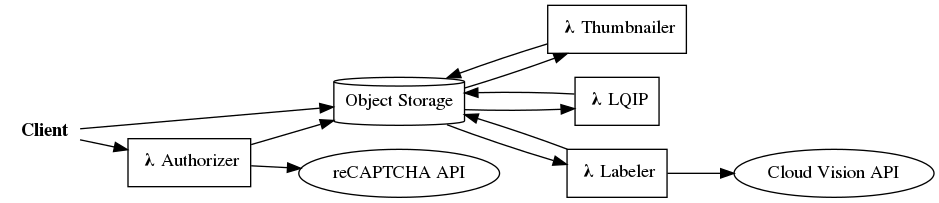
\includegraphics[width=\textwidth]{image-manager-serverless.png}
  \caption{Serverless Image Manager components}
  \label{fig:serverlessArchitecture}
\end{figure}

\begin{figure}[H]
  \centering
  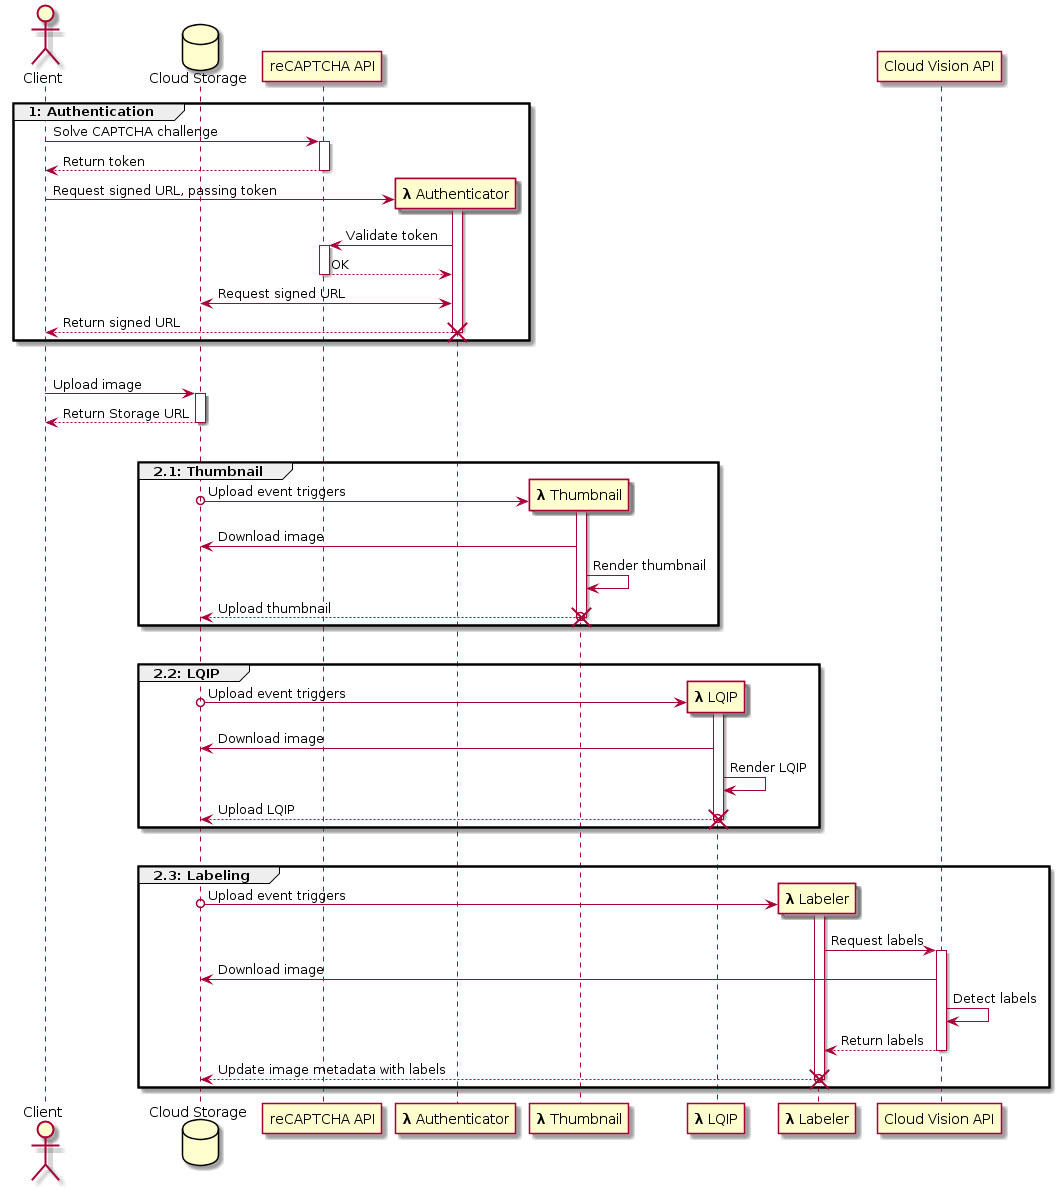
\includegraphics[width=1\textwidth]{sequence-serverless.png}
  \caption{Serverless Image Manager upload sequence (steps 2.1-2.3 run in parallel)}
  \label{fig:serverlessSequence}
\end{figure}

\section{New patterns} \label{sec:newPatterns}

This section lists five new patterns extracted from migration process. The patterns present solutions to problems in Image Manager's serverless design e.g. in places where the serverless implementation performs worse than the original one or fails to provide the same behaviour. In addition we're introducing patterns that could be used to extend the serverless design to further improve its quality or add functionality beyond the original requirements.

\subsection{Async Response} \label{subsec:AsyncResponse}

\textbf{Problem:} Client does not get any feedback from the asynchronous tasks it triggers.

\begin{figure}[h]
  \centering
  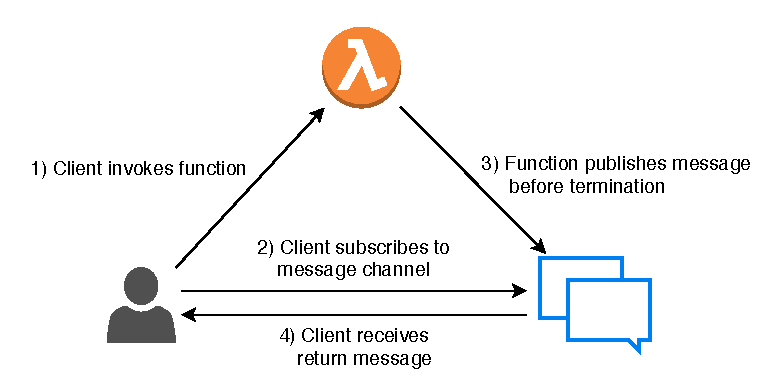
\includegraphics[width=0.7\textwidth]{patterns/async-response.pdf}
  \caption{Async Response}
  \label{fig:asyncResponse}
\end{figure}

\textbf{Solution:} Use a pub/sub channel to notify the client before function termination.

In the pre-migration Image Manager all processing happens in the span of the single upload request. The request blocks and the client will not receive a response before all processing and storage uploads are finished. The serverless Image Manager client on the other hand only receives an acknowledgment of receipt of the original image since image processing is continued asynchronously after the initial Cloud Storage upload. This means the serverless client has no way of notifying the user of a finished processing task. Solving this problem requires a way for the image processing functions to notify the client after they finished with execution.

In more general terms the problem is one of an asynchronously invoked function instance re-establishing communication with the original task initiator, i.e. turning fire-and-forget into something more resembling of request-and-response semantics. As additional complexity, the initiator might not be the actual function invoker but further down the call stack, as in the case of Image Manager where client first activates Cloud Storage which then invokes processing functions.

The Async Response pattern tackles the problem using publish-subscribe messaging. The client, after initiating the task, subscribes to a message channel and waits for notification of the task completion. Conversely the last function responsible for task execution publishes a message to the same channel before terminating. After receiving acknowledgment of task completion the client can dismantle the message channel and proceed to update the the user interface. Instead of a single completion message we could also send status messages during execution for the client to keep track of task progress.

The Async Response can be implemented with any technology that enables publish-subscribe messaging between the client and function: Firebase Realtime Database on Google Cloud or API Gateway Websockets on AWS, for example. One implementation challenge concerns identifying the completion message: how should the message be sent so that it ends up at the right client? One approach is to wrap task initialization in another function that first creates a message channel with an unique identifier and then passes the identifier to both the client and the processing function. This however incurs the overhead of having to pass the channel identifier along each processing step. Another approach is to compute the channel identifier from task payload: in case of Image Manager the channel could be named for example after the uploaded file's name.

\subsection{Task Controller} \label{subsec:taskManager}

\textbf{Problem:} Client has no way of controlling or cancelling an asynchronous task after triggering it.

\begin{figure}[h]
  \centering
  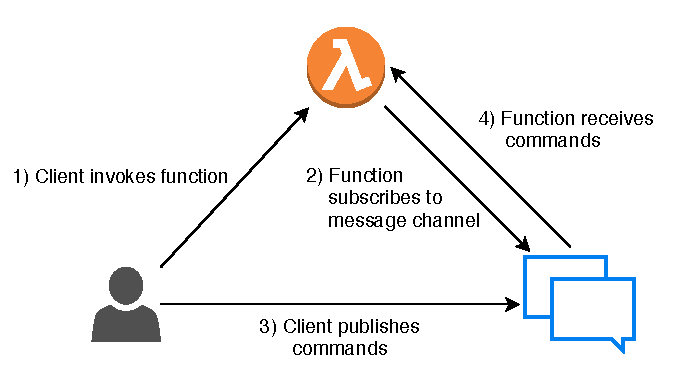
\includegraphics[width=0.65\textwidth]{patterns/task-controller.pdf}
  \caption{Task Controller}
  \label{fig:taskController}
\end{figure}

\textbf{Solution:} Make each function instance open a messaging channel to the client in the beginning of its execution in order to listen to client commands.

Possible future use cases for Image Manager would be to track processing task progress and cancel processing tasks midway. We could for example want to terminate a long-running and expensive batch job if its made redundant before completion, or tweak task parameters after initiating it.

The Task Controller provides a general way for clients to issue commands to function instances mid-execution. The pattern extends the Async Response pattern by turning one-way function-to-client messaging into a two-way channel: instead of just publishing messages at the end of their lifespan, functions also start listening for messages right after initialization.

\subsection{Local Threader} \label{subsec:LocalThreads}

\textbf{Problem:} Scaling an I/O bound operation out to parallel function instances is inefficient since the instances compete of the same I/O resources.

\begin{figure}[h]
  \centering
  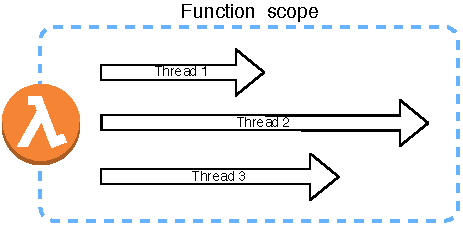
\includegraphics[width=0.55\textwidth]{patterns/local-threader.pdf}
  \caption{Local Threader}
  \label{fig:localThreader}
\end{figure}

\textbf{Solution:} Use local OS threads inside a single function instance to efficiently scale out operations like network requests.

Serverless Image Manager's labeling function is heavily I/O bound since the majority of its execution duration is spent waiting for network requests: first for the labeling request to Cloud Vision API and then for the metadata update request to Cloud Storage (see the sequence diagram in Figure \ref{fig:serverlessSequence}). Scaling this function is therefore inefficient since a larger amount of reserved computing resources does not make network requests finish any faster. In addition as shown in Section \ref{sec:providers}, on some FaaS platforms parallel function instances could end up being allocated on the same physical machine where they share and contest for the same network resources. In fact scaling out instances just to wait for network requests can lead to runaway costs since a waiting function is billed just the same as a processing one; this was discussed in Section \ref{sec:economics} on the economics of serverless.

The Local Threader pattern circumvents the problem by performing I/O-bound operations concurrently inside a single function instance instead of allocating a new instance for each operation. For example in Image Manager's labeling task, Local Threading can be applied to batch image upload events and then send multiple Cloud Vision API requests concurrently inside a single function instance. The pattern takes advantage of the fact that serverless functions, while limited in computing resources and lifespan, are still essentially full-fledged container instances with access to OS threads and processes. For example an AWS Lambda instance can use up to 1024 threads \parencite{awslambda0218}.

The potential cost savings depend largely on the nature of the I/O-bound operation, number of concurrent operations and the way the FaaS platform handles I/O. While an interesting area for future work, optimizing and benchmarking this is outside the scope of the thesis.

\subsection{Prefetcher} \label{subsec:prefetcher}

\textbf{Problem:} Each event handler triggered in response to a single event starts execution by fetching the identical event metadata, resulting in redundant network traffic.

\begin{figure}[h]
  \centering
  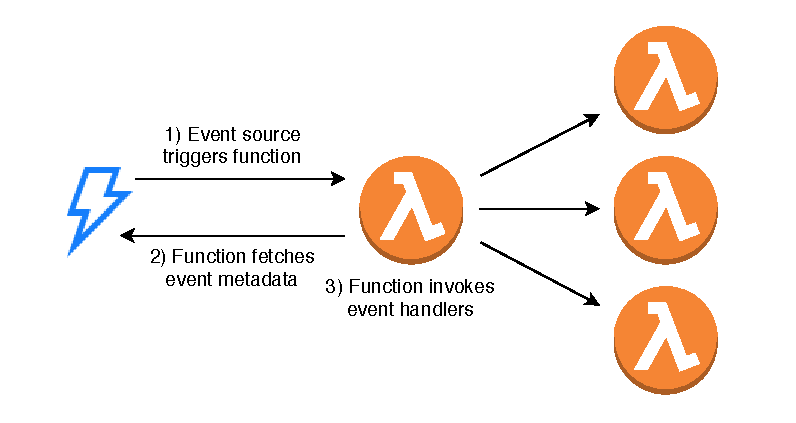
\includegraphics[width=0.75\textwidth]{patterns/prefetcher.pdf}
  \caption{Prefetcher}
  \label{fig:prefetcher}
\end{figure}

\textbf{Solution:} Trigger a single event handling function that fetches event metadata once and then triggers the other event handlers, passing metadata as function payload.

Image Manager's two rendering functions follow largely the same behaviour: triggered by an image upload event emitted from Cloud Storage, they receive the image file URL as input, make a network request to Cloud Storage to fetch the file, render a thumbnail or an LQIP respectively, and finally upload the result to Cloud Storage (see the sequence diagram in Figure \ref{fig:serverlessSequence}). The first step is the same for both functions: the Cloud Storage upload event payload does not include the actual file but just the URL, so all processing functions have to start by downloading the file. In Image Manager's case this is not especially problematic since the FaaS platform and storage service share an internal network. In other cases fetching additional event information could however incur considerable latency or cost overhead in form of network and service charges.

The Prefetcher is an optimization pattern for avoiding expensive duplicate event metadata requests. Its implementation involves adding a new function between the event and its handler functions. Upon event occurrence, the prefetcher function first fetches the metadata and then invokes the actual event handlers, passing the fetched metadata as invocation payload. As a result the event handlers now do not need to separately fetch the extended event metadata. The Event Broadcast pattern (\ref{subsec:EventBroadcast}) can be utilized to avoid coupling the original event handlers with the prefetcher function.

As before with the Local Threading pattern, Prefetcher's efficiency gains are highly dependent on the nature of the metadata request, the number of event handlers as well as on how the FaaS platform handles networking. The pattern is also limited by the maximum function payload size which in AWS Lambda is 6MB for synchronous and 256KB for asynchronous invocations \parencite{awslambda0218}, and in Google Cloud Functions 10MB for both invocation types \parencite{google18cloudFunctions}.

\subsection{Throttled Recursion} \label{subsec:throttledRecursion}

\textbf{Problem:} A spike of recursive function invocations can exceed the platform's maximum concurrency limit.

\begin{figure}[h]
  \centering
  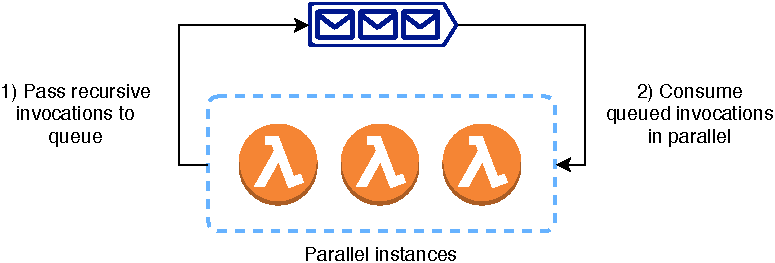
\includegraphics[width=0.75\textwidth]{patterns/throttled-recursion.pdf}
  \caption{Throttled Recursion}
  \label{fig:throttledRecursion}
\end{figure}

\textbf{Solution:} Pass recursive invocations through a message queue in order to throttle their execution.

Another potential future use case for Image Manager is to transform extremely large images or even video material recursively. Using a divide-and-conquer algorithm, a function can split its payload into two or more subtasks and invoke itself recursively until the subtasks become simple enough to solve. The problem with recursion in FaaS however is that the number of concurrent instances can quickly grow out of hand and exceed the platform limit, placing a constraint on recursion depth. We might additionally want to control the rate of recursive branching in order not to overwhelm any potential external services used in subtask solving. A throttled rate of execution can also be desirable to serve as a safety mechanism against infinite loops.

The Throttled Recursion pattern consists of a supplementing the recursive function with a message queue through which each subtask invocation is passed. Instead of directly invoking itself, the recursive function sends its subtasks into the queue and at the same time subscribes to incoming message events. The pattern is similar to the Throttler pattern (\ref{subsec:throttler}) with the exception that here the single function acts both as a producer and as a consumer on the same queue. By adjusting the queue's consumption rate we can control the recursive execution speed. Also now recursion depth is not limited anymore by FaaS concurrency limit but instead by maximum queued messages count which is typically far greater.

\chapter{Evaluation}

Evaluation the outcome of migration process. Estimate the effects on performance and hosting costs. Weigh in on maintainability, testability, developer experience etc.

\chapter{Conclusion}

What can we conclude about the research questions? Mention limitations and further research directions.


\printbibliography

\end{document}
